\documentclass[a4paper,nobib]{tufte-book}

%%
% If they're installed, use Bergamo and Chantilly from www.fontsite.com.
% They're clones of Bembo and Gill Sans, respectively.
%\IfFileExists{bergamo.sty}{\usepackage[osf]{bergamo}}{}% Bembo
%\IfFileExists{chantill.sty}{\usepackage{chantill}}{}% Gill Sans

%\usepackage[protrusion=true,expansion,babel=true]{microtype}

%%
% Just some sample text
\usepackage{lipsum}

%%
% For nicely typeset tabular material
\usepackage{booktabs}
\usepackage{multirow}
\usepackage{adjustbox}
\usepackage{array}

\newcolumntype{L}[1]{>{\noindent\RaggedRight\arraybackslash\hspace{0pt}}p{#1}}
\newcolumntype{R}[1]{>{\noindent\RaggedLeft\arraybackslash\hspace{0pt}}p{#1}}
\newcolumntype{C}[1]{>{\noindent\Centering\arraybackslash\hspace{0pt}}p{#1}}

%%
% For graphics / images
\usepackage{graphicx}
\setkeys{Gin}{width=\linewidth,totalheight=\textheight,keepaspectratio}
\graphicspath{{media/}}

% What
\setcounter{secnumdepth}{3}
\setcounter{tocdepth}{3}

% Bibliography
\usepackage[
style=ieee,
citestyle=numeric-comp,
autocite=inline,
autopunct=true,
backend=biber,
maxbibnames=99,
maxcitenames=2,
mincitenames=1,
]{biblatex}
\addbibresource{bibliography.bib}


%%
% Maths
\usepackage{amsmath}

% Prints a trailing space in a smart way.
\usepackage{xspace}

% Inserts a blank page
\newcommand{\blankpage}{\newpage\hbox{}\thispagestyle{empty}\newpage}

% Referencing
\usepackage[unicode]{hyperref}
\usepackage[nameinlink]{cleveref}

\hypersetup{%
	bookmarksnumbered = true, % Show section numbering in the PDF table of contents. Allows easier browsing of the document
	colorlinks = true, % uncomment this line if you prefer colored hyperlinks (e.g., for onscreen viewing)
%	pdfborder = {0 0 0},
	bookmarksdepth = subsection,
%	citecolor = DarkGreen,
%	linkcolor = DarkBlue,
%	urlcolor = DarkGreen,
}

%\AtBeginDocument{%
%	\hypersetup{
%		pdfauthor={\plainauthor}
%		pdftitle={\plaintitle},
%	}%
%}

\usepackage[binary-units=true]{siunitx}

% Modifications to the default tufte template to make it more applicable to a thesis
% Credit goes to Tiffany Tseng, lalider, see https://github.com/lalider/tufte-latex-thesis

\usepackage[parfill]{parskip}

% remove paragraph indentation
\makeatletter
% Paragraph indentation and separation for normal text
\renewcommand{\@tufte@reset@par}{%
	\setlength{\RaggedRightParindent}{0.0pc}%
	\setlength{\JustifyingParindent}{0.0pc}%
	\setlength{\parindent}{0pc}%
	\setlength{\parskip}{\baselineskip}%
}
\@tufte@reset@par

% Paragraph indentation and separation for marginal text
\renewcommand{\@tufte@margin@par}{%
	\setlength{\RaggedRightParindent}{0.0pc}%
	\setlength{\JustifyingParindent}{0.0pc}%
	\setlength{\parindent}{0.0pc}%
	\setlength{\parskip}{10pt}%
}
\makeatother

\titleformat{\section}%
[hang]% shape
{\normalfont\Large}% format applied to label+text
{\thesection}% label
{1em}% horizontal separation between label and title body
{}% before the title body
[]% after the title body

%\titlespacing*{\section}{0pt}{3.5ex plus 1ex minus .2ex}{2.3ex plus .2ex}
%\titlespacing*{\subsection}{0pt}{3.25ex plus 1ex minus .2ex}{1.5ex plus.2ex}
\titlespacing*{\section}{0pt}{30pt}{20pt}
\titlespacing*{\subsection}{0pt}{20pt}{5pt}


% Disable adding empty pages without a purpose (not intended for printing in a book format...)
\makeatletter
\def\cleardoublepage{
	\clearpage%
}
\makeatother

% Acronyms
\usepackage{acro}
\acsetup{
	use-id-as-short,
	make-links=false,
	case-sensitive=false,
	patch/floats=false,
	patch/caption=false,
	patch/tabularx=false
}
\DeclareAcronym{FDIR}{short=FDIR,long={Fault Detection, Isolation and Recovery}}
\DeclareAcronym{ADCS}{short = ADCS, long = {Attitude Determination and Control Subsystem}}
\DeclareAcronym{COMMS}{short = COMMS, long = {Communications}}
\DeclareAcronym{EPS}{short = EPS, long = {Electrical Power Subsystem}}
\DeclareAcronym{OBC}{short = OBC, long = {On-Board Computer}}
\DeclareAcronym{OBDH}{short = OBDH, long = {On-Board Data Handling}}
\DeclareAcronym{OBSW}{short = OBSW, long = {On-Board Software}}
\DeclareAcronym{OPS}{short = OPS, long = {Operations}}
\DeclareAcronym{SYE}{short = SYE, long = {Systems Engineering}}
\DeclareAcronym{SU}{short = SU, long = {Science Unit}}
\DeclareAcronym{EMC}{short = EMC, long = {Electromagnetic Compatibility}}
\DeclareAcronym{CDR}{short = CDR, long = {Critical Design Review}}
\DeclareAcronym{GS}{short = GS, long = {Ground Station}}
\DeclareAcronym{TC}{short = TC, long = Telecommands}
\DeclareAcronym{TM}{short = TM, long = Telemetry}
\DeclareAcronym{RF}{short = RF, long = RadioFrequency}
\DeclareAcronym{CCSDS}{short = CCSDS, long = {The Consultative Committee for Space Data Systems}}
\DeclareAcronym{ISM}{short = ISM, long = {Industrial, Scientific, Medical}}
\DeclareAcronym{COTS}{short = COTS, long = {Commercial Off-The-Shelf}}
\DeclareAcronym{PCDU}{short = PCDU, long = {Power Conditioning \& Distribution Unit}}
\DeclareAcronym{MPPT}{short = MPPT, long = {Maximum Power Point Tracking}}
\DeclareAcronym{ECSS}{short = ECSS, long = {European Cooperation for Space Standardization}}
\DeclareAcronym{PUS}{short = PUS, long = {Packet Utilisation Standard}}
\DeclareAcronym{UHF}{short = UHF, long = {Ultra-High Frequency}}
\DeclareAcronym{LEO}{short = LEO, long = {Low Earth Orbit}}
\DeclareAcronym{PDMS}{short = PDMS, long = {Polydimethylsiloxane}}
\DeclareAcronym{PA}{short = PA, long = {Product Assurance}}
\DeclareAcronym{PCB}{short = PCB, long = {Printed Circuit Board}}
\DeclareAcronym{GMAT}{short = GMAT, long = {General Mission Analysis Tool}}
\DeclareAcronym{MRAM}{short = MRAM, long = {Magnetoresistive Random-Access Memory}}
\DeclareAcronym{CAN}{short = CAN, long = {Controller Area Network}}
\DeclareAcronym{MCU}{short = MCU, long = {microcontroller}, extra={MicroController Unit}}
\DeclareAcronym{RTOS}{short = RTOS, long = {Real-Time Operating System}}
\DeclareAcronym{SAVOIR}{short = SAVOIR, long = {Space AVionics Open Interface aRchitecture}}
\DeclareAcronym{YAMCS}{short = YAMCS, long = {Yet Another Mission Control System}}
\DeclareAcronym{COBS}{short = COBS, long = {Consistent Overhead Byte Stuffing}}
\DeclareAcronym{SRAM}{short = SRAM, long = {Static Random Access Memory}}
\DeclareAcronym{I2C}{short = {I\textsuperscript{2}C}, long = {Inter-Integrated Circuit}}
\DeclareAcronym{ETL}{short = ETL, long = {Embedded Template Library}}
\DeclareAcronym{HAL}{short = HAL, long = {Hardware Abstraction Library}}
\DeclareAcronym{IDE}{short = IDE, long = {Integrated Development Environment}}
\DeclareAcronym{USB}{short = USB, long = {Universal Serial Bus}}
\DeclareAcronym{UART}{short = UART, long = {Universal Asynchronous Serial Bus}}
\DeclareAcronym{FMEA}{short = FMEA, long = {Failure Mode and Effects Analysis}}
\DeclareAcronym{FMECA}{short = FMECA, long = {Failure Mode, Effects and Criticality Analysis}}
\DeclareAcronym{HSIA}{short = HSIA, long = {Hardware/Software Interaction Analysis}}
\DeclareAcronym{XTCE}{short = XTCE, long = {XML Telemetric and Command Exchange}}
\DeclareAcronym{RAMS}{short = RAMS, long = {Reliability, Availability, Maintainability and Safety}}
\DeclareAcronym{MAIV}{short = MAIV, long = {Maintenance, Assembly, Integration and Verification}}
\DeclareAcronym{IC}{short = IC, long = {Integrated Circuit}}
\NewDocumentCommand\draft{m}{%
	\textcolor[HTML]{bf616a}{#1}%
}

\makeatletter
\newcommand\footurl@[1]{\footnote{\url@{#1}}}
\DeclareRobustCommand{\footurl}{\hyper@normalise\footurl@}

\newcommand\foothref@[2]{\href@{#1}{#2}\footnote{\url@{#1}}}
\def\Hy@foothref#{%
	\hyper@normalise\foothref@
}
\DeclareRobustCommand*{\foothref}[1][]{%
	\begingroup
	\setkeys{href}{#1}%
	\@ifnextchar\bgroup\Hy@foothref{\hyper@normalise\foothref@}%
}
\makeatother

% Transitions
\AtBeginDocument{
\colorlet{invalid}{MaterialAmber900}
\colorlet{unexpected}{MaterialRed900}
}

\def\unchecked{\textcolor{MaterialGrey800}{\texttt{Unchecked}}}
\def\ok{\texttt{OK}}
\def\unexpected{\textcolor{unexpected}{\texttt{Unexpected\_Value}}}
\def\hilim{\textcolor{unexpected}{\texttt{Above\_High\_Limit}}}
\def\lolim{\textcolor{unexpected}{\texttt{Below\_Low\_Limit}}}
\def\invalid{\textcolor{invalid}{\texttt{Invalid}}}
\def\ar{ \( \rightarrow \) }

\makeatletter

\makeatother

\NewAcroTemplate[list]{glossary}{%
	\begin{description}
		\acronymsmapF{%
			\item[\sffamily\textbf{\acrowrite{short}}] \acrowrite{long}%
			\acroifanyT {foreign,extra} {~(}%
			\acrowrite {foreign}%
			\acroifallT {foreign,extra} {,~}%
			\acrowrite {extra}%
			\acroifanyT {foreign,extra} {)}%
			\acropagefill%
			\acropages%
				{ \acrotranslate {page} \nobreakspace }%
				{ \acrotranslate {pages} \nobreakspace }%
		}%
		{ \item \AcroRerun{list} }%
		\end {description}
	}

% Various utilities
\usepackage{tabularx}
\usepackage[singlelinecheck=false]{caption}
\usepackage{subcaption}
\usepackage{comment}

% Generates the index
\usepackage{makeidx}
\makeindex

\usepackage{tikz}
\usepackage{pgfplots}
\pgfplotsset{compat = 1.3}
\usetikzlibrary{pie}
\usepackage{physics}
\let\Re=\relax
\let\Im=\relax

% Colours
\definecolor{off}{HTML}{e53935}
\definecolor{on}{HTML}{43a047}
\usepackage{xcolor-solarized}
\usepackage{xcolor-material}
\usepackage{colortbl}

%\usepackage{todonotes}
\usepackage{enumitem}
\usepackage[absolute,overlay]{textpos}

% Code
\usepackage{minted}
\usepackage{xpatch,letltxmacro}
\LetLtxMacro{\cminted}{\minted}
\let\endcminted\endminted
\xpretocmd{\cminted}{\RecustomVerbatimEnvironment{Verbatim}{BVerbatim}{}}{}{}
\definecolor{mintedbg}{rgb}{0.95,0.95,0.93}
\setminted{
	bgcolor=mintedbg,
	tabsize=2
}
\setminted[text]{baselinestretch=0.8}

% Git magic
\makeatletter
\write18{git log --pretty='format:\@percentchar Creset\@percentchar s' --no-merges -1 > \jobname.git1.tmp}
\write18{git rev-parse --short HEAD > \jobname.git2.tmp}
\def\gitcommit{\input{\jobname.git2.tmp}\unskip}
\def\gitcommitmessage{\input{\jobname.git1.tmp}\unskip}
\makeatother

% Smart citations

\makeatletter

%\def\blx@imc@mkbibquote{\blx@enquote}

\newbibmacro*{cite:title}{%
  \printtext[bibhyperref]{%
    \printfield[citetitle]{labeltitle}}%
  \finentry}

\newbibmacro*{cite:shorthand}{%
	\printtext[bibhyperref]{\printfield{shorthand}}}

\newbibmacro*{cite:full}{%
	\iffieldundef{shorthand}
	{\printnames{labelname}%
		\setunit*{\printdelim{nametitledelim}}%
		\usebibmacro{cite:title}}%
	{\usebibmacro{cite:shorthand}}}

\newbibmacro*{cite:marginnote}{%
	\marginnote{%
		% \mkbibbrackets should be used here probably
		[%
			\printfield{labelprefix}%
			\printfield{labelnumber}%
		]
		\usebibmacro{cite:full}%
	}%
}

\DeclareCiteCommand{\dualcite}[\mkbibbrackets]
  {\usebibmacro{cite:init}%
   \usebibmacro{prenote}}
  {\usebibmacro{citeindex}%
   \usebibmacro{cite:marginnote}%
   \usebibmacro{cite:comp}}%
  {}
  {\usebibmacro{cite:dump}%
   \usebibmacro{postnote}}

\def\tuftecite{
	\iffootnote{footnote}{text}
}

% Patching commands that enter information in margins, so that we can detect which
% citation should be used
\newtoggle{inmargin}
\pretocmd{\marginpar}{\toggletrue{inmargin}}{}{}
\apptocmd{\@xympar}{\togglefalse{inmargin}}{}{}
\pretocmd{\@tufte@float}{\toggletrue{inmargin}}{}{}
\pretocmd{\end@tufte@float}{\togglefalse{inmargin}}{}{}
\pretocmd{\@tufte@margin@float}{\toggletrue{inmargin}}{}{}
\pretocmd{\end@tufte@margin@float}{\togglefalse{inmargin}}{}{}

\def\autocite{%
	\iftoggle{inmargin}\parencite\dualcite%
}

% Tufte disables subparagraphs. This brings them back.
\renewcommand\subparagraph{\@startsection{subparagraph}{5}{\parindent}%
	{3.25ex \@plus1ex \@minus .2ex}%
	{-1em}%
	{\hspace{1em}\normalfont\normalsize\itshape}}

% \acuse command that also adds the current page
%\NewAcroTemplate{fdirthesisempty}{}
%\NewAcroCommand\acusepage{m}{}
\let\acusepage\acuse

\makeatother

% Greek
\usepackage[utf8]{inputenc}
\usepackage[greek,english]{babel}
\usepackage{alphabeta}
\let\textlozenge\undefined
\usepackage{gfsartemisia-euler}
\NewDocumentCommand{\g}{m}{\foreignlanguage{greek}{#1}}
%\usepackage{hyphenation-greek}
%\input{hyphenation-el.tex}

%%
% Book metadata
\title{Design of Fault Detection, Isolation and Recovery in the AcubeSAT nanosatellite\thanks{AcubeSAT}}
\author[Konstantinos Kanavouras]{Konstantinos Kanavouras}
\publisher{\ensuregreek{Αριστοτέλειο Πανεπιστήμιο Θεσσαλονίκης}}

\begin{document}

% Front matter
%\frontmatter

% r.1 blank page
%\blankpage

% r.3 full title page
\makeatletter
\renewcommand{\maketitle}{%
	\newpage
	\global\@topnum\z@% prevent floats from being placed at the top of the page
	\begingroup
	\setlength{\parindent}{0pt}%
	\setlength{\parskip}{4pt}%
	\let\@@title\@empty
	\let\@@author\@empty
	\let\@@date\@empty
	\thispagestyle{empty}
	\begin{fullwidth}
		\vfill
		\begin{center}
			\href{https://www.auth.gr/}{
\includegraphics[width=.8\textwidth]{auth_logo_text}}\par
			\vspace{1cm}
			\LARGE\textsc{Διπλωματικη Εργασια}\par
			\vspace{6ex}
			\hrule
			\vspace{4ex}
			\Huge\textbf{Σχεδιασμός μηχανισμού Ανίχνευσης, Απομόνωσης και Αντιμετώπισης Βλαβών}\\[1ex]
			\LARGE\textbf{στον}\\
			\Huge\textbf{Νανοδορυφόρο AcubeSAT}\par
			\vspace{2.7ex}
			\hrule

			\vspace{4ex}

			\Large
			\begin{tabular}{ll}
				\emph{Συγγραφέας:} & \href{https://github.com/kongr45gpen}{Κωνσταντίνος \textsc{Καναβουρας} \normalsize (\fontfamily{pplx}\selectfont 8824)}
				\\[1.5ex]
				\emph{Επιβλέπων:} & \href{http://ee.auth.gr/en/school/faculty-staff/electronics-computers-department/hatzopoulos-alkiviadis/}{Καθ. Αλκιβιάδης \textsc{Χατζοπουλος}}
			\end{tabular}

			\vspace{6ex}

			\large \textit{Η διπλωματική εργασία κατατίθεται για \\ την εκπλήρωση των υποχρεώσεων για λήψη διπλώματος}\\[0.3cm] % University requirement text
			\textit{στην}\\[0.4cm]
			\href{https://www.eng.auth.gr/en/home.html}{Πολυτεχνική Σχολή}
			\\
			\href{https://ee.auth.gr/en/}{Τμήμα Ηλεκτρολόγων Μηχανικών \& Μηχανικών Υπολογιστών}
			\\[1cm] % Research group name and department name

			\vspace{6ex}

			{\large \today}\\[4cm] % Date

		\end{center}
		\vfill
	\end{fullwidth}
	\endgroup
	\thispagestyle{plain}% suppress the running head
	\tuftebreak% add some space before the text begins
	\@afterindentfalse\@afterheading% suppress indentation of the next paragraph
}
\makeatother
\maketitle

% v.4 copyright page
\newpage
\begin{fullwidth}
~\vfill
\thispagestyle{empty}
\setlength{\parindent}{0pt}
\setlength{\parskip}{\baselineskip}
Copyright \copyright\ \the\year\ \thanklessauthor

\par\smallcaps{Δημοσιευτηκε απο το \thanklesspublisher}

\par\smallcaps{\href{https://github.com/kongr45gpen/thesis-latex}{Https://GitHub.com/Kongr45gpen/Thesis-Latex}}

\justify

\par Αυτή η εργασία χορηγείται με άδεια Creative Commons Αναφορά Δημιουργού 4.0 Διεθνές (CC BY 4.0) (η ``Άδεια'')· το κείμενο του παρόντος δεν επιτρέπεται να χρησιμοποιηθεί παρά μόνο με βάση την Άδεια. Για να δείτε ένα αντίγραφο αυτής της άδειας, επισκεφτείτε το
\url{https://creativecommons.org/licenses/by/4.0/legalcode.el}, ή δείτε μια "αναγνώσιμη από άνθρωπο" σύνοψη στο \url{https://creativecommons.org/licenses/by/4.0/deed.el}.\index{license}

\par Το AcubeSAT project εκτελείται με την υποστήριξη του Education Office του \href{https://www.esa.int/}{Ευρωπαϊκού Οργανισμού Διαστήματος}, στα πλαίσια του \href{https://www.esa.int/Education/CubeSats_-_Fly_Your_Satellite/}{προγράμματος Fly Your Satellite!}.

\par Οι απόψεις που εκφράζονται στο παρόν από τους συγγραφείς δεν μπορούν \smallcaps{σε καμια περιπτωση να θεωρηθει πως εκφραζουν} την επίσημη άποψη, ή υποστήριξη, του Ευρωπαϊκού Οργανισμού Διαστήματος.

\par\textit{Rendered on \today{} (\texttt{\gitcommit}: \gitcommitmessage)}
\end{fullwidth}

% r.5 contents
\tableofcontents

\begin{fullwidth}
\listoffigures

\listoftables

%\chapter*{List of Acronyms}
%\acuseall%
\bgroup
\setlength\parskip{1ex}
\printacronyms[pages={display=all,seq/use=false},]
\egroup

\end{fullwidth}

% r.9 introduction
\cleardoublepage

\chapter*{Περίληψη}

%This sample book discusses the design of Edward Tufte's

\justify
Το διάστημα δεν είναι ένα φιλόξενο περιβάλλον: αν και η σημερινή τεχνολογία έχει επιτρέψει τη λειτουργία χιλιάδων τεχνητών δο\-ρυ\-φό\-ρων σε τροχιά γύρω από τη γη, οι νανοδορυφόροι που χαρακτηρίζονται ως “CubeSats” έχουν ένα ποσοστό αποτυχίας κοντά στο 50\%. Τα χαμηλά κόστη, η έλλειψη αυστηρών τεχνικών προδιαγραφών και η έλλειψη ανοιχτής τεχνικής βιβλιογραφίας συχνά αυξάνει τα ρίσκα για τα εκπαιδευτικά, επιστημονικά και εμπορικά CubeSat. Αυτή η εργασία ερευνά μία απλή παραμετροποιήσιμη αρχιτεκτονική Ανίχνευσης, Απομόνωσης και Αντιμετώπισης Βλαβών (“FDIR”) που βασίζεται σε Ευρωπαϊκά πρότυπα και πρωτόκολλα, ευρέως χρησιμοποιούμενα στον τομέα της αεροδιαστημικής. Αυτή η δομή διόρθωσης σφαλμάτων, μαζί με τη συνοδευόμενη υλοποίηση σε κώδικα, μπορεί να χρησιμοποιηθεί από οποιαδήποτε αποστολή CubeSat για να αυξηθεί η αξιοπιστία του σχεδιασμού και να μειωθεί η πιθανότητα αποτυχίας, μέσω της αυτόνομης αντιμετώπισης βλαβών κατά την πτήση. Η εργασία επίσης περιλαμβάνει γενικές πληροφορίες σχετικά με την αξιοπιστία των CubeSat, και εξερευνά το λογισμικό και υλικό που χρησιμοποιείται για να υλοποιηθεί το προτεινόμενο FDIR στην αποστολή AcubeSAT, η οποία βρίσκεται υπό σχεδιασμό από φοιτητές του Αριστοτελείου Πανεπιστημίου Θεσσαλονίκης.

\chapter*{Abstract}

%\begin{fullwidth}
\begin{center}
	\large Konstantinos Kanavouras
	\par
	\vspace{2ex}
	\Large\textbf{Design of Fault Detection, Isolation and Recovery}\\
	\large\textbf{in the}\\
	\Large\textbf{AcubeSAT NanoSatellite}\par
	\draft{university, supervisor etc.}
\end{center}
%\end{fullwidth}

%This sample book discusses the design of Edward Tufte's
%books\parencite{Tufte2001,Tufte1990,Tufte1997,Tufte2006}.
\justify
Space is not a welcoming environment; while the aerospace engineering community has managed to reliably operate thousands of satellites in orbit, CubeSats, the most popular class of nanosatellite, only have a 50\% success rate. Low costs, lack of strict technical requirements and scarcity of publicly available documentation often drives up the risks for educational, scientific and commercial CubeSats. This thesis investigates a configurable and modular Fault Detection, Isolation and Recovery (FDIR) architecture that uses the ECSS Packet Utilisation Standard. This FDIR concept, along with the provided open-source software implementation, can be used by CubeSat missions to increase the reliability of their design and chances of mission success, by autonomously responding to on-board errors. The thesis also includes background information regarding CubeSat reliability, and explores the software and hardware used to implement the proposed FDIR design on the AcubeSAT mission, currently under design by students of the Aristotle University of Thessaloniki.


%%
% Start the main matter (normal chapters)
\mainmatter


\chapter{Εισαγωγή}

\section{Επιστημονική Περιοχή}
\draft{1-2 pages}

\section{Σκοπός και Συνεισφορά της Εργασίας}

\section{Διάρθωση και Δομή}

\chapter{Αξιοπιστία στα συστήματα CubeSat}
\label{sec:fdir}


%\newthought{The pages} of a book are usually divided into three major
%sections: the front matter (also called preliminary matter or prelim), the
%main matter (the core text of the book), and the back matter (or end
%matter).

%\newthought{The front matter} of a book refers to all of the material that
%comes before the main text.  The following table from shows a list of
%material that appears in the front matter of
%along with its page number.  Page numbers that appear in parentheses refer
%to folios that do not have a printed page number (but they are still
%counted in the page number sequence).



\section{Εισαγωγή στην Αεροδιαστημική Δυναμική}
cubesat reliablity \autocite{durou_hierarchical_fault_2002}

\section{Νανοδορυφόροι \& CubeSat}

\section{Αξιοπιστία CubeSat}

\acf{FDIR}

\chapter{Η αποστολή AcubeSAT}

\section{Η αποστολή}
\draft{Here we write the history of the project and a description of the mission and the satellite...}

\section{Υποσυστήματα}

Ο νανοδορυφόρος AcubeSAT είναι τεχνικά και οργανωτικά χωρισμένος σε 11 διαφορετικές υποομάδες ή \textbf{υποσυστήματα}, κάθε μία από τις οποίες είναι υπεύθυνη για ένα διαφορετικό τμήμα του δορυφόρου, και αποτελείται από \SIrange{2}{9}{} αφοσιωμένα μέλη.

Στις επόμενες ενότητες παρουσιάζεται μια σύντομη εισαγωγή στη λειτουργία και το σχεδιασμό κάθε υποσυστήματος. Καθώς η διαδικασία σχεδιασμού συστημάτων και \acl{PA} είναι %\ensuregreek{εγ\-γε\-νώς}
\g{εγγενώς}
συνδεδεμένη με τη λειτουργία όλων των υποσυστημάτων, \g{αναφέρονται} επίσης οι λεπτομέρειες που αφορούν το \acs{FDIR}. Για πιο λεπτομερείς πληροφορίες, ο αναγνώστης ενθαρρύνεται να ανατρέξει στην \foothref{https://acubesat.spacedot.gr/subsystems/}{ιστοσελίδα του AcubeSAT}, ή στα δημοσίως διαθέσιμα \foothref{https://gitlab.com/acubesat/documentation/cdr-public}{έγγραφα του \ac{CDR}}.

\subsection{\acf{ADCS}}
\label{sec:adcs}

Η υποομάδα του \ac{ADCS} είναι υπεύθυνη για τον έλεγχο του \textbf{προσανατολισμού} του δορυφόρου σε τροχιά. Αυτό επιτυγχάνεται με τη χρήση μιας σειράς ενεργοποιητών, που προέρχονται έτοιμοι από την αγορά (\ac{COTS}): μία πλακέτα 3 αξόνων και έναν τροχός αντίδρασης 1 άξονα, σε συνδυασμό με αισθητήρες για τον προσδιορισμό της περιστροφής του δορυφόρου (1 γυροσκόπιο και 2 μαγνητόμετρα) και αλγορίθμους φιλτραρίσματος \& ελέγχου. \autocite{DDJF_AOCS,velentzas_design_attitude_2021}

Το \ac{ADCS} μπορεί να λειτουργήσει με τα εξής διαφορετικά ``προφίλ στόχευσης'' (pointing profiles) για να καλύψει διαφορετικές λειτουργικές ανάγκες:
\begin{enumerate}
	\item \textbf{Λειτουργία Σταθεροποίησης} (Detumbling), όπου ο δορυφόρος προσπαθεί να φτάσει τη γωνιακή του ταχύτητα κοντά στο 0, για να εξασφαλίσει μια αξιόπιστη ραδιοζεύξη, να αποτρέψει την αποκόλληση εξαρτημάτων και να επιτρέψει αργότερα την ευκολότερη ανάκτηση του επιθυμητού προσανατολισμού.
	
	Η λειτουργία Σταθεροποίησης υλοποιείται με τον απλούστερο δυνατό τρόπο, χρησιμοποιώντας μόνο το ένα από τα 2 μαγνητόμετρα και έναν απλό αλγόριθμο ελέγχου. Ενεργοποιείται όταν δεν υπάρχει ανάγκη εφαρμογής κάποιου άλλου ή όταν η γωνιακή ταχύτητα του νανοδορυφόρου είναι επικίνδυνα υψηλή. Στο AcubeSAT, το προφίλ αυτό εφαρμόζεται στην \emph{Ασφαλή Λειτουργία}, στη \emph{Λειτουργία Εκκίνησης} και στη \emph{Λειτουργία Πειράματος}.
	
	\item \textbf{Στόχευση στο Ναδίρ} (Nadir Pointing), όπου ο δορυφόρος \g{στρέ\-φει} την πλευρά \(+X\) ώστε να κοιτάζει προς τη Γη. Αυτό το προφίλ χρησιμοποιείται κατά τη διάρκεια της \emph{Κανονικής Λειτουργίας} σε περάσματα πάνω από τον Σταθμό Βάσης, όπου η κατευθυντική κεραία χρειάζεται άμεση ορατότητα.
	
	\item \textbf{Στόχευση στον Ήλιο} (Sun Pointing), όπου ο δορυφόρος \g{στρέ\-φει} δύο πλευρές προς τον ήλιο με γωνία πρόσπτωσης \SI{45}{\degree}, προ\-κει\-μέ\-νου να μεγιστοποιηθεί η είσοδος των ηλιακών πάνελ. Αυτό το προφίλ χρησιμοποιείται κατά τη διάρκεια της \emph{Κανονικής Λειτουργίας}, ανάμεσα στα περάσματα από το Σταθμό Βάσης, προκειμένου να εξασφαλιστεί θετικός προϋπολογισμός ισχύος.
\end{enumerate}

\begin{margintable}
	\centering
	\caption[Μέγιστες τιμές σφαλμάτων ADCS μετά τη σταθεροποίηση]{Μέγιστες τιμές σφαλμάτων \ac{ADCS} μετά τη σταθεροποίηση}
	\label{tab:adcsape}
	\begin{tabular}{@{}ll@{}}
		\toprule
		Σφάλμα                      & Τιμή                    \\ \midrule
		Απόλυτη Ακρίβεια Στόχευσης & \( < \SI{30}{\degree} \) \\
		Απόλυτη Ακρίβεια Γνώσης    & \( < \SI{1}{\degree} \) 
	\end{tabular}
\end{margintable}

Οι επιδόσεις του \ac{ADCS} μπορούν να αξιολογηθούν με μετρικές όπως αυτές που παρουσιάζονται στον \Cref{tab:adcsape}.

\subsection{\acf{COMMS}}

Το υποσύστημα communications (τηλεπικοινωνιών) είναι υπεύθυνο για τη μετάδοση δεδομένων μεταξύ της Γης και του δορυφόρου σε τροχιά. Τα μεταδιδόμενα δεδομένα χωρίζονται σε 3 διαφορετικές κατηγορίες\autocite{DDJF_TTC}:
\begin{itemize}
	\item \textbf{\acf{TC}}: Εντολές από τη Γη προς το δορυφόρο. Μπορούν να χρησιμοποιηθούν για να ζητήσουν πληροφορίες ή για να εκτελέσουν συγκεκριμένες ενέργειες στο CubeSat.
	\item \textbf{\acf{TM}}: Πληροφορίες που αποστέλλονται από τον δορυφόρο προς τη Γη, που συνήθως περιλαμβάνουν ζωτικές πληροφορίες, όπως τιμές αισθητήρων, κατάσταση συστήματος, τρέχουσα ώρα και συμβάντα.
	\item \textbf{Επιστημονικά δεδομένα}: Τα επιστημονικά δεδομένα που παράγονται από το ωφέλιμο φορτίο (payload). Αυτά είναι τα δεδομένα με τον μεγαλύτερο όγκο και αντιπροσωπεύουν τα κύρια επιστημονικά αποτελέσματα της αποστολής.
\end{itemize}

Είναι σημαντικό να αναφερθεί ότι η τροχιά του δορυφόρου επιτρέπει μόνο μια πολύ μικρή διάρκεια ορατότητας από τον Σταθμό Βάσης (\acf{GS}) κάθε μέρα, αυξάνοντας τις ανάγκες για αυτονομία επί του σκάφους και τη σημασία μιας σωστά εφαρμοσμένης μεθόδου \acs{FDIR}.

\begin{marginfigure}
	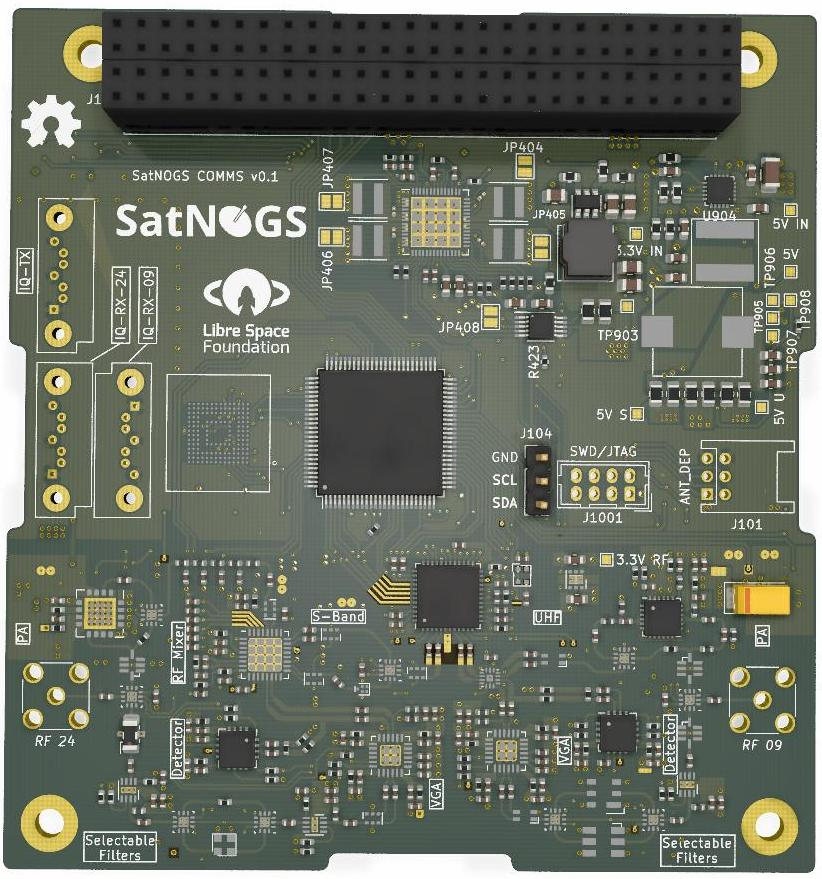
\includegraphics{satnogs-comms}
	\caption{Η πλακέτα SatNOGS COMMS}
\end{marginfigure}

Το κύριο συστατικό του υποσυστήματος \acs{COMMS} είναι η πλακέτα \textbf{SatNOGS COMMS} \autocite{surligas_satnogscomms_2021}, ένας \acs{RF} πομποδέκτης ανοικτού κώδικα που αναπτύσσεται από την \href{https://libre.space/}{LibreSpace Foundation}, βασισμένη στα τηλεπικοινωνιακά πρότυπα \acs{CCSDS}.

Η επικοινωνία πραγματοποιείται με τη χρήση 2 ζωνών συχνοτήτων στην περιοχή \acs{ISM}, \SI{436.5}{\mega\hertz} και \SI{2.425}{\giga\hertz}, μέσω μίας κεραίας διπόλων και μίας κατευθυντικής επιφανειακής κεραίας (patch antenna). Η χρήση των συχνοτήτων \acs{ISM} επιτρέπει την εύκολη ραδιοερασιτεχνική πρόσβαση στο δορυφόρο. Η πρώτη (\acs{UHF}) ζώνη εκπέμπει επίσης ένα περιοδικό σήμα \textbf{beacon} (ραδιοφάρος), που περιέχει κρίσιμες πληροφορίες σχετικά με την κατάσταση του δορυφόρου.

Το υποσύστημα τηλεπικοινωνιών είναι επίσης υπεύθυνο για την ανάλυση ηλεκτρομαγνητικής συμβατότητας (\acs{EMC}), καθώς και για το σχεδιασμό και την κατασκευή του Σταθμού Βάσης. Ο τελευταίος θα αποτελέσει μέρος του \textbf{SatNOGS}\autocite{white_overview_satellite_2018}, ενός παγκόσμιου δικτύου δορυφορικών επίγειων σταθμών που βασίζεται σε ανοικτές τεχνολογίες και ανοικτά δεδομένα.

\subsection{\acf{EPS}}
Το  \ac{EPS} is the subsystem responsible for the generation, distribution and storage of electrical power of the spacecraft. It is a critical aspect of the spacecraft due to the direct dependence of all subsystems to the high power needs of many CubeSat subsystems, and is theorised to be the most common reason for CubeSat failure.\autocite{langer_reliability_cubesats_2016}

Το \ac{EPS} είναι το υποσύστημα υπεύθυνο για την παραγωγή, κατανομή και αποθήκευση ηλεκτρικής ενέργειας στον δορυφόρο. Είναι ένα κρίσιμο κομμάτι του CubeSat, λόγω της άμεσης εξάρτησης και των σχετικά αυξημένων ενεργειακών αναγκών πολλών υποσυστημάτων του, και θεωρείται πως είναι ο πιο πιθανός λόγος αποτυχίας των CubeSat σε τροχιά. \autocite{langer_reliability_cubesats_2016}

Το AcubeSAT έχει επιλέξει έναν συνδυασμό από \ac{COTS} προϊόντα για το \ac{EPS}:\autocite{DDJF_SYS}
\begin{itemize}
	\item Τα \textbf{ηλιακά πάνελ} (solar panels) αγοράζονται από την EnduroSat. 4 πάνελ διάστασης 3U καλύπτουν τις \(X\) και \(Y\) πλευρές, και ένα πάνελ 1U καλύπτει την \(-Z\) πλευρά.
	\item Η μονάδα \textbf{ελέγχου και διανομής ισχύος} (\ac{PCDU}) αγοράζεται από την NanoAvionics και προσφέρει 10 προστατευμένα κανάλια με 4 διαφορετικές τιμές τάσης, καθώς και 4 μετατροπείς \ac{MPPT}.
	\item The \textbf{battery pack}, also procured from NanoAvionics, contains 4 18650 Li-Ion cells in a 2S2P\footnote{2 series, 2 parallel} configuration.
	\item Οι \textbf{μπαταρίες}, επίσης αγορασμένες από τη NanoAvionics, αποτελούνται από 4 στοιχεία ιόντων λιθίου μορφής 18650.
\end{itemize}

\begin{margintable}
	\caption{Προϋπολογισμός ισχύος AcubeSAT σε κανονική λειτουργία}
	\label{tab:power_budget}
	\begin{tabularx}{\linewidth}{@{}lX@{}}
		\toprule
		\textbf{Καταναλωτής}            & \textbf{Ισχύς}            \\ \midrule
		\acs{ADCS}          & \SI{1.10}{\watt} \\
		\acs{COMMS}         & \SI{0.85}{\watt} \\
		\acs{EPS}           & \SI{0.99}{\watt} \\
		\acs{OBC}           & \SI{0.12}{\watt} \\
		\acs{SU}            & \SI{0.25}{\watt} \\ \midrule
		Σύνολο               & \SI{3.30}{\watt} \\
	    Μέση παραγόμενη ισχύς & \SI{4.24}{\watt} \\ \bottomrule
	\end{tabularx}
\end{margintable}

\FloatBarrier
\begin{comment}
A dynamic approach is taken with regards to power budget calculation:
\begin{compactenum}
	\item The in-orbit power generation is calculated for the duration of the mission using the \textbf{STK} software, taking into account satellite orientation, pointing profiles and eclipse, with a \SI{1}{\minute} resolution.
	\item The power consumption of the system is calculated on average for each different operational mode.
	\item \acs{MPPT} efficiencies and battery charge level are calculated for each timepoint, assuming worst-case thermal and electrical conditions
	\item A system-wide 10\% margin is applied to the results
\end{compactenum}


We have created a Python library consolidating the above steps\footurl{https://gitlab.com/acubesat/eps/power-budget} and producing the necessary outputs to prove the adequacy of the design.
\end{comment}


\begin{figure*}[h]
%	\begin{subfigure}[b]{.45\textwidth}
	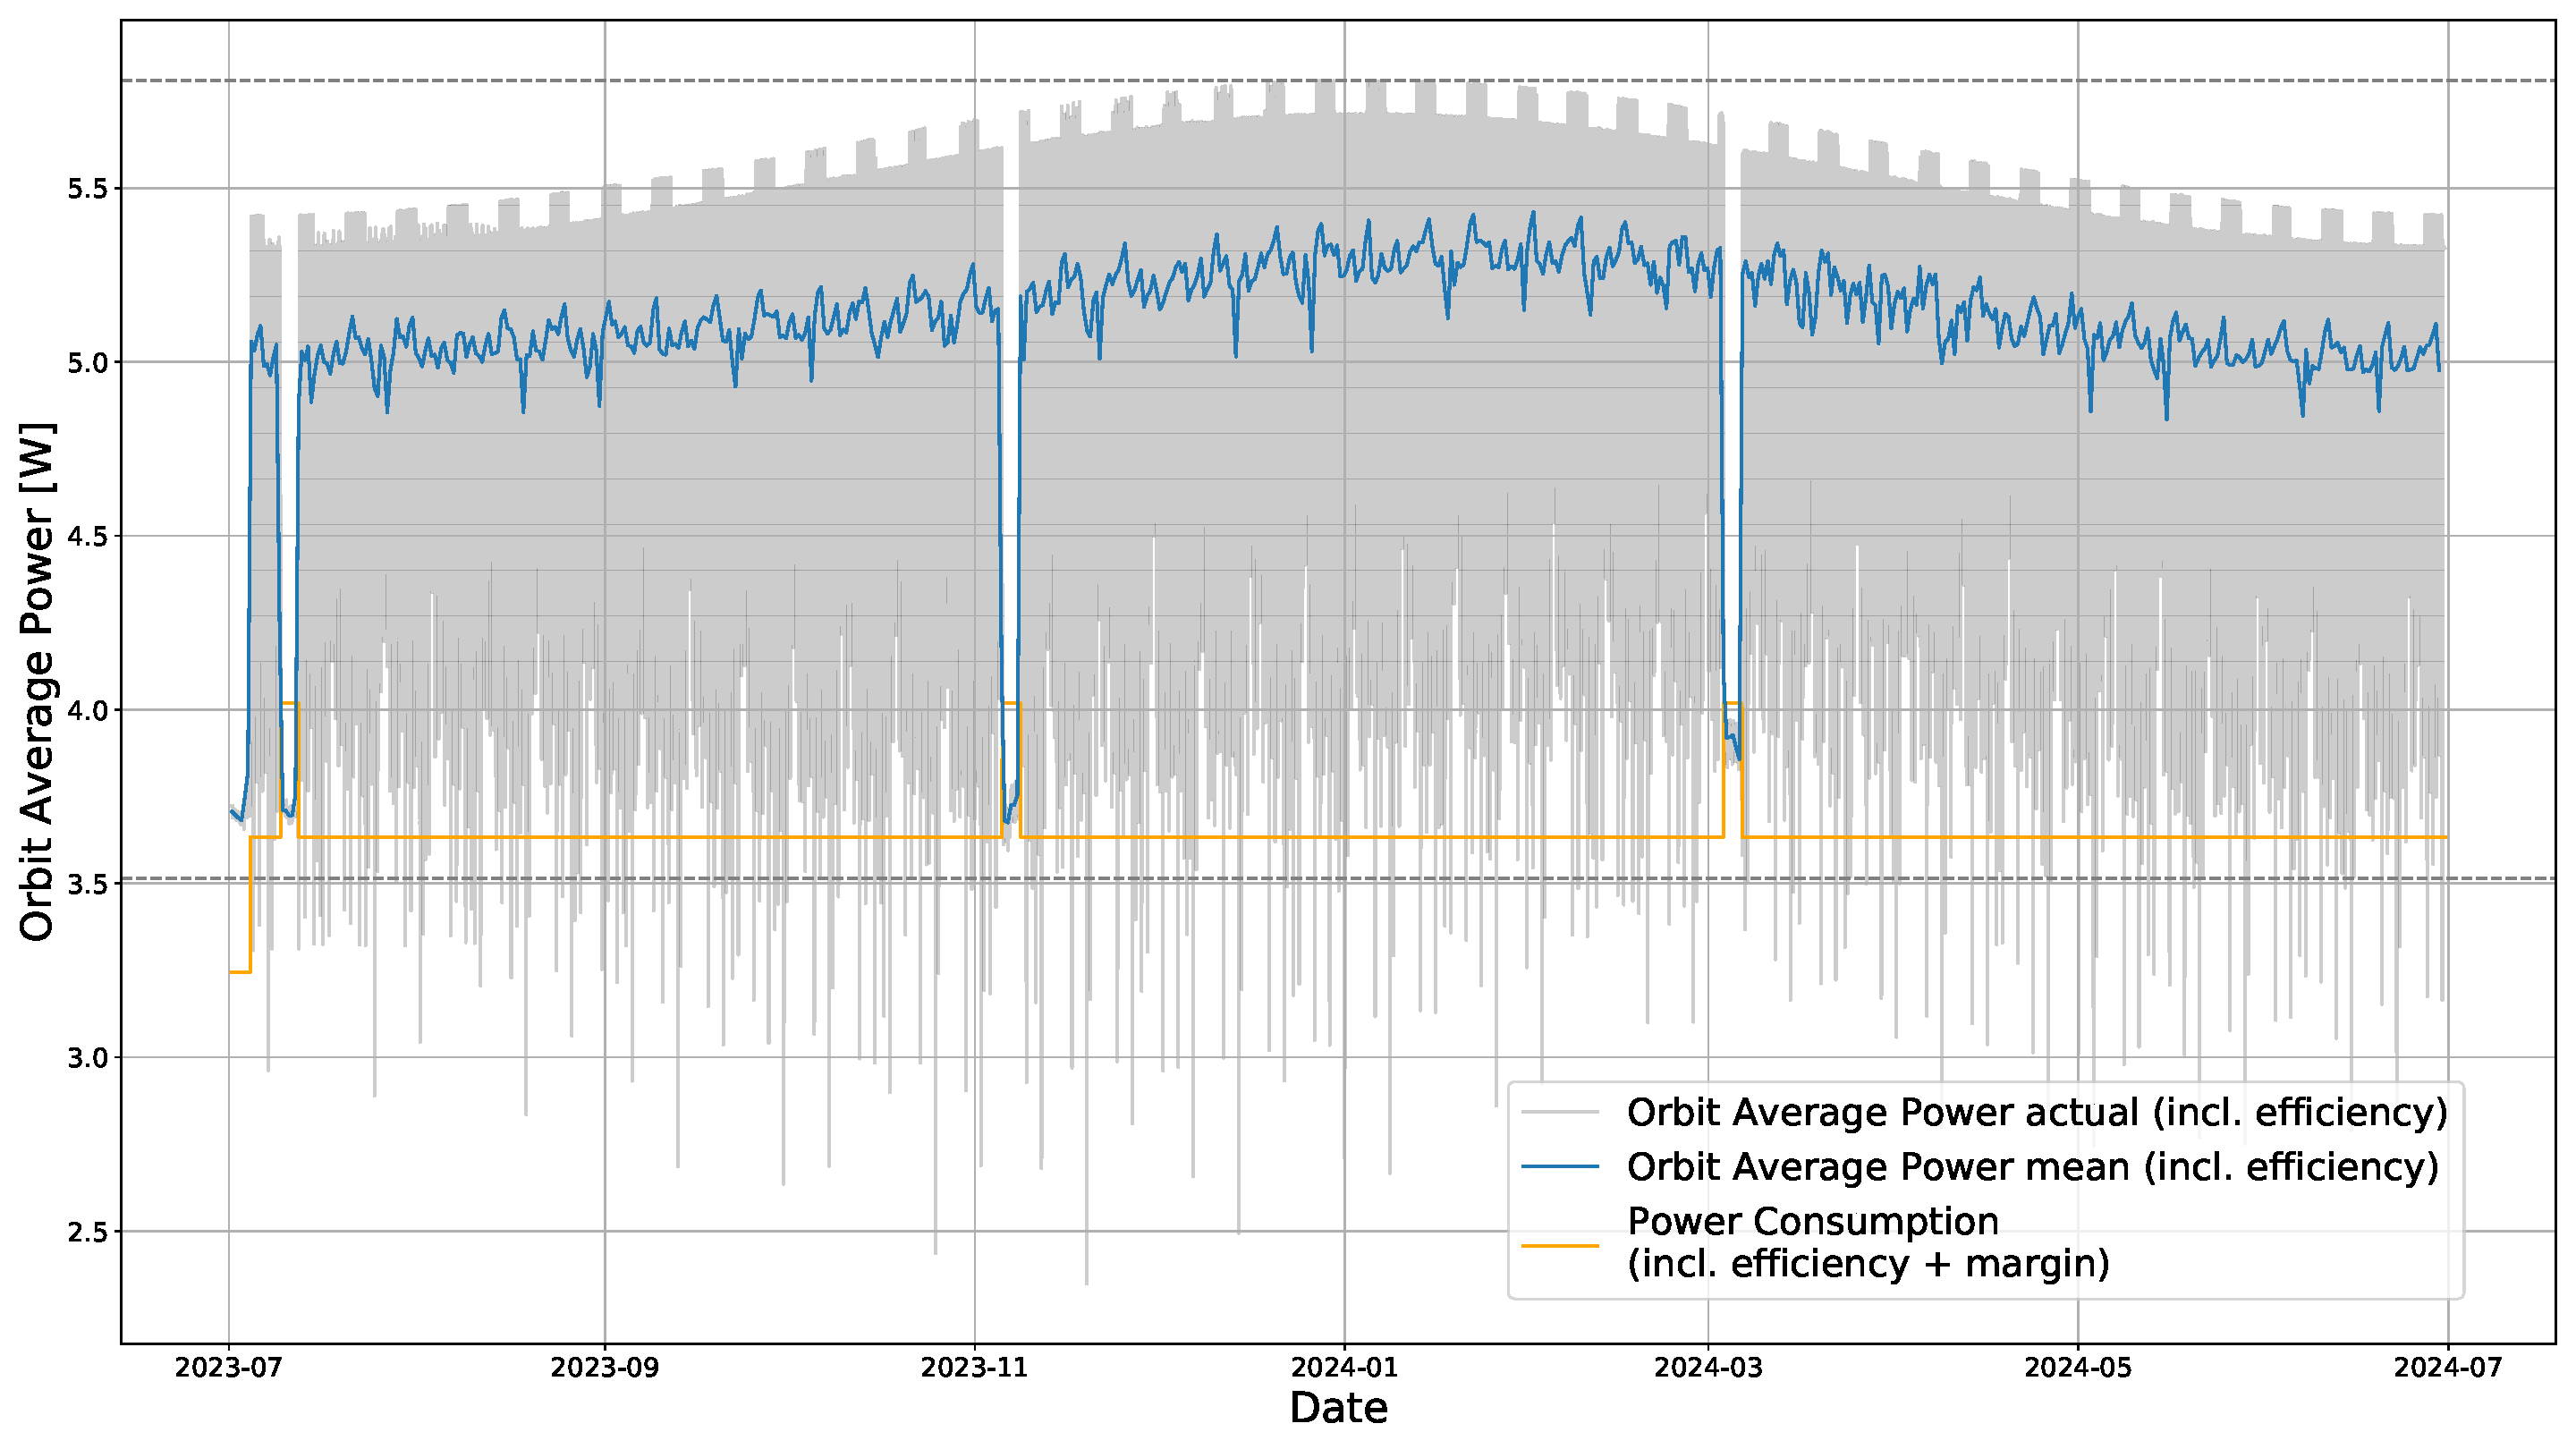
\includegraphics[height=4cm]{Sun Pointing 11:00.total.pdf}
%	\end{subfigure}
	\hfill
%	\begin{subfigure}[b]{.45\textwidth}
	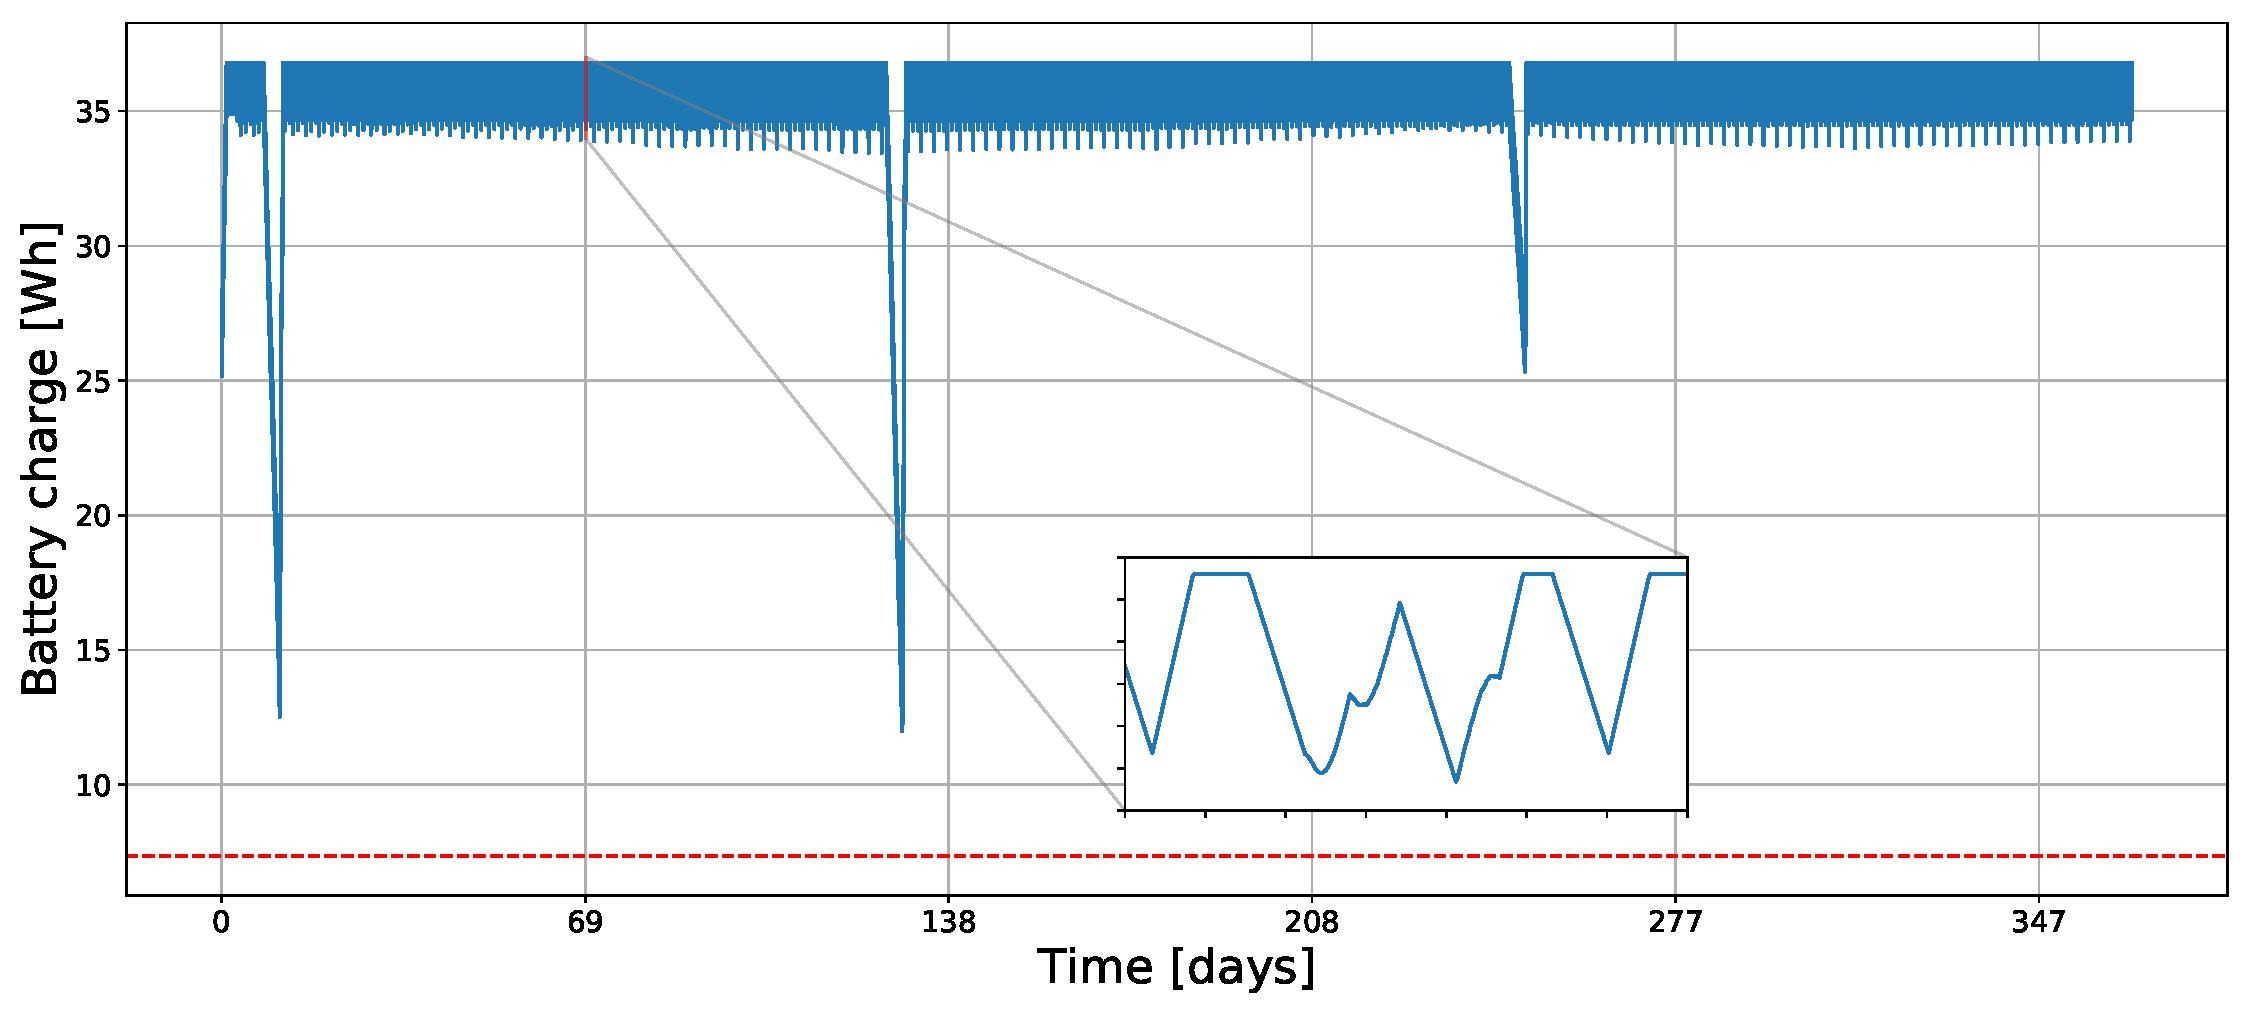
\includegraphics[height=4cm]{Sun Pointing 11:00.discharge.pdf}
%	\end{subfigure}
%	\includegraphics[width=.45\textwidth]{/home/kongr45gpen/Pictures/jeka8ara kapoglis.png}

	\caption[Δυναμική ανάλυση προϋπολογισμού ισχύος]{Δυναμική ανάλυση προϋπολογισμού ισχύος. Αριστερά: Κατανάλωση \& παραγωγή ισχύος στην τροχιά. Δεξιά: Επίπεδο εκφόρτισης μπαταρίας κατά τη διάρκεια της αποστολής}
\end{figure*}

\subsection{\acf{OBDH}}
\label{sec:obdh}

Το υποσύστημα \ac{OBDH} είναι υπεύθυνο για το σχεδιασμό των διεπαφών δεδομένων του διαστημικού σκάφους, καθώς και για το σχεδιασμό της πλακέτας \textbf{\acf{OBC}}, η οποία είναι επιφορτισμένη με τον έλεγχο των βασικών λειτουργιών του AcubeSAT. \autocite{DDJF_OBDH}

Η πλακέτα \ac{OBC} περιέχει τα βασικά εργαλεία για την εξασφάλιση της αυτονομίας, και βασίζεται σε έναν ανθεκτικό στην ακτινοβολία μικροελεγκτή \foothref{https://www.microchip.com/wwwproducts/en/SAMV71Q21RT}{Microchip SAMV71Q21RT}, και μια μνήμη \acs{MRAM} που χρησιμοποιείται για την αποθήκευση κρίσιμων δεδομένων. Η πλακέτα φιλοξενεί επίσης τον "εγκέφαλο" του υποσυστήματος \ac{ADCS}, ως μέτρο εξοικονόμησης χώρου.

\begin{marginfigure}
	\centering
	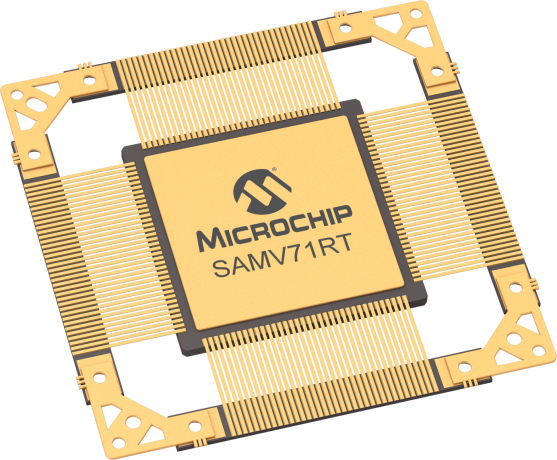
\includegraphics[width=.7\textwidth]{SAMV71Q21RT}
	\caption{Ο μικροελεγκτής \texttt{SAMV71Q21RT}}
	\label{fig:samv71}
\end{marginfigure}

AcubeSAT's data interface is using a cold-redundant \ac{CAN} bus to facilitate cross-subsystem communication, selected due to its robustness and reliability. \autocite{bouwmeester_survey_implementation_2017} AcubeSAT boards implement the PC/104 mechanical interface.\autocite{PC104}

Η διεπαφή δεδομένων μεταξύ των υποσυστημάτων του AcubeSAT χρησιμοποιεί ένα \ac{CAN} bus σε \textbf{ψυχρό πλεονασμό} (cold redundancy), το οποίο επιλέχθηκε λόγω της υψηλής αξιοπιστίας του. \autocite{bouwmeester_survey_implementation_2017} Οι πλακέτες του AcubeSAT ικανοποιούν τις μηχανικές απαιτήσεις του προτύπου PC/104. \autocite{PC104}

\subsection{\acf{OBSW}}


Το υποσύστημα \ac{OBSW} είναι υπεύθυνο για το σχεδιασμό και την ανάπτυξη του λογισμικού του νανοδορυφόρου. Η γλώσσα που επιλέχθηκε να χρησιμοποιηθεί στους 4 μικροελεγκτές είναι μια περιορισμένη μορφή της \textbf{C++}, και ο κώδικας ελέγχεται από μια σειρά προτύπων, στατικών αναλυτών και unit tests.\autocite{DDJF_OBSW} Όλο το λογισμικό εκτελείται επάνω στο λειτουργικό σύστημα πραγματικού χρόνου Free\acs{RTOS}.


\subsection{\acf{OPS}}

Το υποσύστημα Operations είναι υπεύθυνο για το σχεδιασμό των λειτουργιών \& διαδικασιών του διαστημικού σκάφους και για τη διασφάλιση της λειτουργικότητας, της δυνατότητας ελέγχου και της παρατηρησιμότητας του δορυφόρου πριν και κατά τη διάρκεια της τροχιάς του.

Κατά τη διάρκεια της αποστολής, το AcubeSAT μπορεί να βρίσκεται σε μία από τις ακόλουθες\textbf{λειτουργίες συστήματος}:\autocite{MDO}
\begin{itemize}
	\item \textbf{Λειτουργία Εκτόξευσης} (Launch/Off mode): Ο δορυφόρος είναι πλήρως απενεργοποιημένος και κανένα υποσύστημα δεν λαβάνει ισχύ. Αυτή η λειτουργία αναπαριστά την κατάσταση του διαστημικού σκάφους μέσα στον "deployer", όπου δεν επιτρέπεται η ενεργοποίηση κανενός ηλεκτρονικού στοιχείου,\autocite[req. 3.3.3]{CDS13} και το CubeSat πρέπει να βρίσκεται σε πλήρη αδράνεια.
	
	\item \textbf{Λειτουργία Εκκίνησης} (Commissioning mode): Αυτή η λειτουργία ξεκινάει μόλις ο CubeSat εξέλθει από τον deployer, δηλαδή όταν ολοκληρωθεί η εκτόξευση. Περιλαμβάνει τις αρχικές ενέργειες εκκίνησης του διαστημικού σκάφους, συμπεριλαμβανομένης της εκτύλιξης της κεραίας, και της μείωσης της γωνιακής ταχύτητας. Σε αυτήν τη λειτουργία δεν παράγονται επιστημονικά δεδομένα.
	
	\item \textbf{Κανονική Λειτουργία} (Nominal mode): Εδώ θα βρίσκεται ο δορυφόρος τον περισσότερο χρόνο. Εκτός από τις απαραίτητες λειτουργίες αυτονομίας και τη φόρτιση της μπαταρίας, το CubeSat θα μεταδίδει επίσης τηλεμετρία και επιστημονικά δεδομένα. Εω δεν πραγματοποιείται καμία επιστημονική εργασία, εκτός από τυχόν ελέγχους υγείας. Η κανονική λειτουργία είναι επίσης η μόνη λειτουργία κατά την οποία ο δορυφόρος εκτελεί στόχευση στον ήλιο ή στο ναδίρ (\Cref{sec:adcs}).
	
	\item \textbf{Επιστημονική Λειτουργία} (Science mode): Εδώ πραγματοποιείται το κύριο πείραμα και παράγονται τα επιστημονικά δεδομένα. Αυτή η λειτουργία περιλαμβάνει τη δράση του υδραυλικού συστήματος, τη λειτουργία του τσιπ μικρορευστομηχανικής, την καλλιέργεια των κυττάρων και την περιοδική λήψη εικόνων με τη χρήση του μικροσκοπίου.
	
	Το AcubeSAT έχει χωρίσει την επιστημονική λειτουργία σε \textbf{3 διαφορετικές φάσεις}, που ονομάζονται υπο-πειράματα \(\alpha\), \(\beta\) και \(\gamma\), διαρκούν 72 ώρες το καθένα και εκτελούνται σε διαφορετικά χρονικά σημεία της αποστολήςμ ώστε να διερευνηθεί η χρονική εξάρτηση των παρατηρούμενων αποτελεσμάτων.
	
	\item \textbf{Ασφαλής Λειτουργία} (Safe mode): Συνηθίζεται τα διαστημικά συστήματα να περιλαμβάνουν μια \emph{ασφαλή λειτουργία},\autocite[385]{aguirre_introduction_space_2013} όπου το διαστημικό σκάφος απενεργοποιεί όλα τα μη απαραίτητα συστήματα και διαδικασίες, προκειμένου να ανταποκριθεί σε σημαντικές δυσλειτουργίες που δεν μπορούν να διορθωθούν αυτομάτως. Η ασφαλής λειτουργία προορίζεται ως μια καλά καθορισμένη και καλά δοκιμασμένη λειτουργία, η οποία είναι εύκολη στη συντήρηση και μειώνει τον κίνδυνο οποιασδήποτε καταστροφικής βλάβης.
	
	Στον AcubeSAT, η λειτουργικότητα του διαστημικού σκάφους είναι σημαντικά μειωμένη και το προφίλ στόχευσης προσπαθεί να πετύχει μόνο σταθεροποίηση. Ωστόσο, η επικοινωνία \ac{UHF} και η μετάδοση του περιοδικού beacon εξακολουθούν να είναι ενεργές για λόγους παρατηρησιμότητας.
\end{itemize}

\begin{table*}[h]
	\centering
	\caption{Σύνοψη της λειτουργικότητας του AcubeSAT σε διαφορετικές Λειτουργίες Συστήματος}
	\label{tab:acubesatmodes}
	\begin{tabular}{@{}llllll@{}}
		\toprule
		Υποσύστημα    & Εκτόξευση & Εκκίνηση & Κανονική                 & Επιστημονική        & Ασφαλής             \\ \midrule
		\acs{ADCS}  & \color{off} Off    & Σταθεροποίηση     & \color{on} Στόχευση                & Σταθεροποίηση     & Σταθεροποίηση       \\
		\acs{COMMS} & \color{off} Off    & \acs{UHF} μόνο & \color{on} \acs{UHF} και S-Band    & \acs{UHF} μόνο & \acs{UHF} μόνο   \\
		\acs{EPS}   & \color{off} Off    & \color{on} On             & \color{on} On                      & \color{on} On             & \color{on} On               \\
		\acs{OBC}   & \color{off} Off    & \color{on} On             & \color{on} On                      & \color{on} On             & \color{on} On               \\
		\acs{SU}    & \color{off} Off    & \color{off} Off            & Συντήρηση \& δεδομένα & \color{on} On             & Συντήρηση \\ \bottomrule
	\end{tabular}
	\vspace{1em}
\end{table*}


Κάθε λειτουργία συνδέεται με ένα διάγραμμα \textbf{λειτουργικής ροής}, το οποίο δείχνει μια υψηλού επιπέδου περιγραφή των διαδικασιών που εκτελούνται κατά τη διάρκειά της.\autocite{acubesat_functional_2021}

\begin{figure}
	\centering
	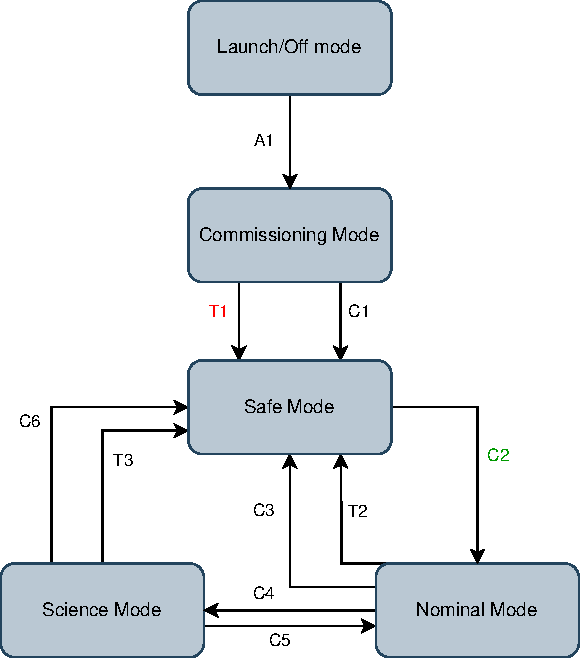
\includegraphics[width=.6\textwidth]{AcubeSAT_System_Modes}
	\caption[][3cm]{Όλες οι μεταβάσεις μεταξύ των Λειτουργιών Συστήματος}
	\label{fig:transitions}
\end{figure}


\subsection{Structural}

Το υποσύστημα Structural έχει αναλάβει:
\begin{itemize}
	\item Την ανάλυση και η διαμόρφωση του \ac{COTS} σκελετού 3U (\Cref{fig:structure}) που στεγάζει όλα τα εξαρτήματα του CubeSat και είναι κατασκευασμένος από αλουμίνιο. Οι αναλύσεις δονήσεων είναι ιδιαίτερα σημαντικές, καθώς διερευνούν κατά πόσο ο CubeSat μπορεί να αντέξει τα μηχανικά φορτία κατά την εκτόξευση.
	\item Τον πλήρη σχεδιασμό, κατασκευή και συναρμολόγηση του \textbf{δοχείου πειράματος} και του ενσωματωμένου σε αυτό πλαστικού "unibody" (\Cref{fig:container}).
\end{itemize}

\begin{marginfigure}
	\centering
	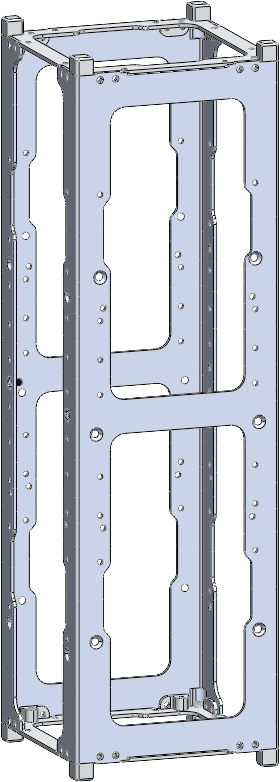
\includegraphics[width=.5\textwidth]{structure}
	\caption{Ο \acs{COTS} σκελετός του CubeSat}
	\label{fig:structure}
\end{marginfigure}

\subsection{\acf{SYE}}

The \acl{SYE} subteam serves as the technical authority for the satellite. It is responsible for coordinating the developments and interfaces between subsystems, ensuring the conformance to standards and technical requirements, and identifying \& resolving all issues arising from the complex multi-discipline design of the CubeSat.

Additionally, the \ac{SYE} team is responsible for some specific technical developments that do not belong in any of the other subsystems, such as \ac{RAMS}, \ac{FMEA}, harnessing and the \acl{MAIV} plan.

Η υποομάδα του \acl{SYE} λειτουργεί ως τεχνική αρχή του δορυφόρου. Είναι υπεύθυνη για το συντονισμό των εργασιών και της επικοινωνίας μεταξύ των υποσυστημάτων, τη συμμόρφωση με τα πρότυπα και τις τεχνικές προδιαγραφές, καθώς και τον εντοπισμό \& την επίλυση όλων των ζητημάτων που προκύπτουν από τον πολύπλοκο σχεδιασμό ενός δορυφορικού συστήματος.

Επιπλέον, η ομάδα \ac{SYE} είναι υπεύθυνη για ορισμένα τεχνικά κομμάτια που δεν ανήκουν σε κανένα από τα άλλα υποσυστήματα, όπως την ανάλυση αξιοπιστίας (\acs{RAMS}), την ανάλυση αποτυχιών \& αποτελεσμάτων τους (\ac{FMEA}), την καλωδίωση και το πλάνο κατασκευής \& δοκιμών (\acs{MAIV}).

\subsection{\acf{SU}}

Η υποομάδα \acl{SU} είναι υπεύθυνη για τη σχεδίαση και την υλοποίηση του επιστημονικού φορτίου της αποστολής, δηλαδή τη μελέτη της επιδράσεων του περιβάλλοντος Χαμηλής Γήινης Τροχιάς (\ac{LEO}) σε ζυμομύκητες.

Το επιστημονικό φορτίο αποτελείται από τα ακόλουθα λειτουργικά μέρη: \autocite{DDJF_PL}
\begin{compactitem}
	\item Το \textbf{δοχείο πειράματος}, μια δομή αλουμινίου μεγέθους σχεδόν 2U, σε τυπική ατμοσφαιρική πίεση και σχεδιασμένη να φιλοξενεί όλα τα όργανα του πειράματος. Το δοχείο φιλοξενεί επίσης ένα μονόσωμα (\textbf{"unibody"}) που στηρίζει μηχανικά όλα τα εξαρτήματα.
	\item Ένα \textbf{τσιπ μικρορευστομηχανικής} (microfluidic chip) βασισμένο σε \ac{PDMS}, που φιλοξενεί 384 θαλάμους ικανούς να εξετάσουν 190 διαφορετικά στελέχη των μυκητών \emph{Saccharomyces Cerevisiae} για κάθε υποπείραμα.
	\item Ένα \textbf{fluidic system} που αποτελείται από 2 αντλίες, 14 ηλεκτρομαγνητικές βαλβίδες και 3 σακούλες υγρών.
	\begin{marginfigure}
		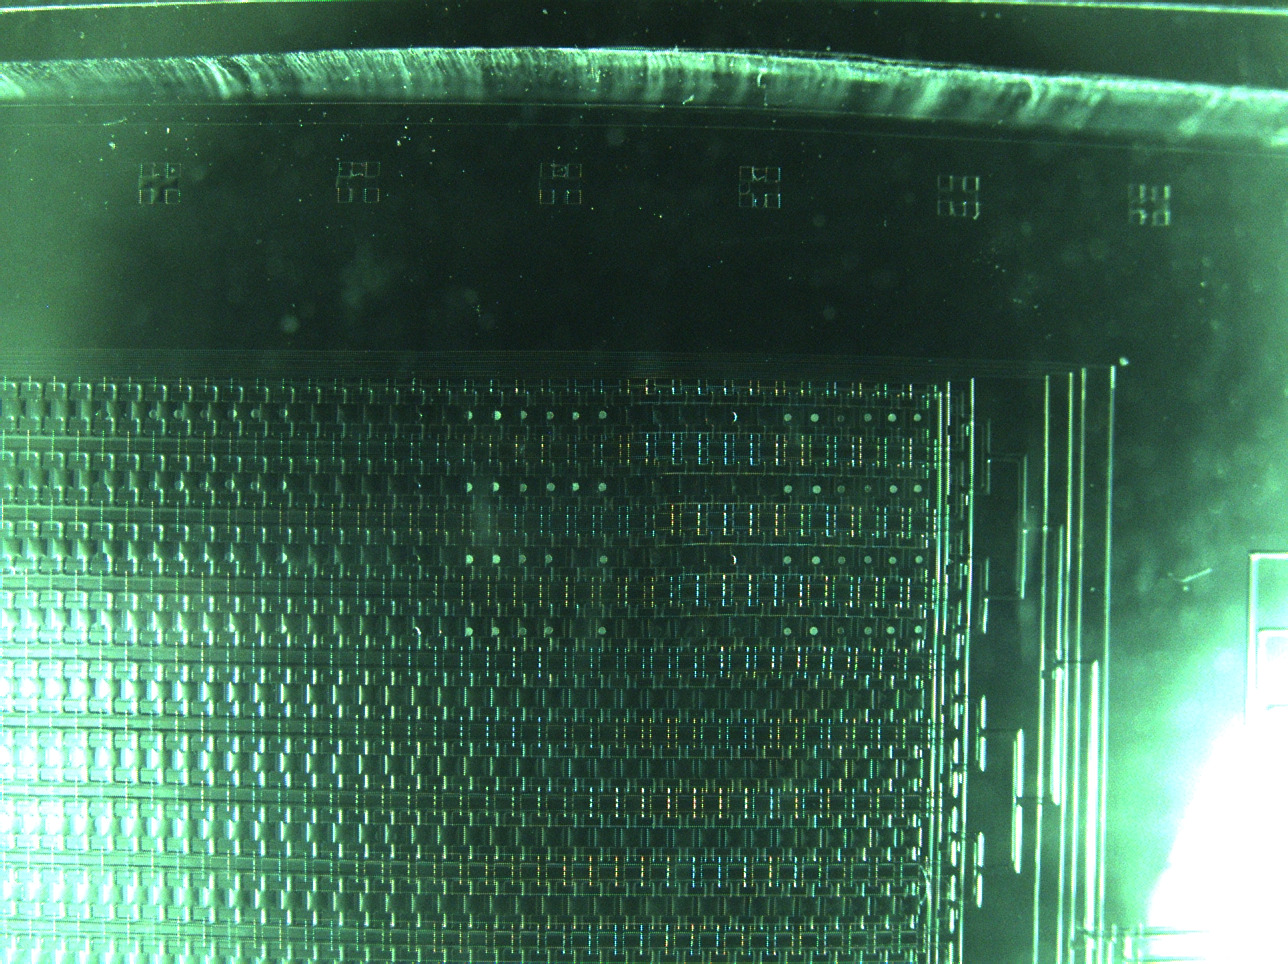
\includegraphics{chipFluor}
		\caption[Παράδειγμα παραγόμενης εικόνας]{Παράδειγμα παραγόμενης εικόνας (\parencite{DDJF_PL})}
		\label{fig:chip_fluor}
	\end{marginfigure}
	\item Ένα \textbf{οπτικό σύστημα} που λειτουργεί ως μικροσκόπιο, το οποίο περιέχει μια κάμερα και μια σειρά από λαμπτήρες, φίλτρα και ένα φακό
	\item Έναν αριθμός \textbf{θερμαντικών σωμάτων} για τον αυστηρό έλεγχο των θερμοκρασιών λειτουργίας των εξαρτημάτων
	\item Έναν αριθμός πλεοναζόντων \textbf{αισθητήρων} για περιβαλλοντικές μετρήσεις
	\item Μία πλακέτα που περιέχει τον μικροελεγκτή και τα υπόλοιπα εξαρτήματα ελέγχου
\end{compactitem}

\begin{marginfigure}
	\centering
	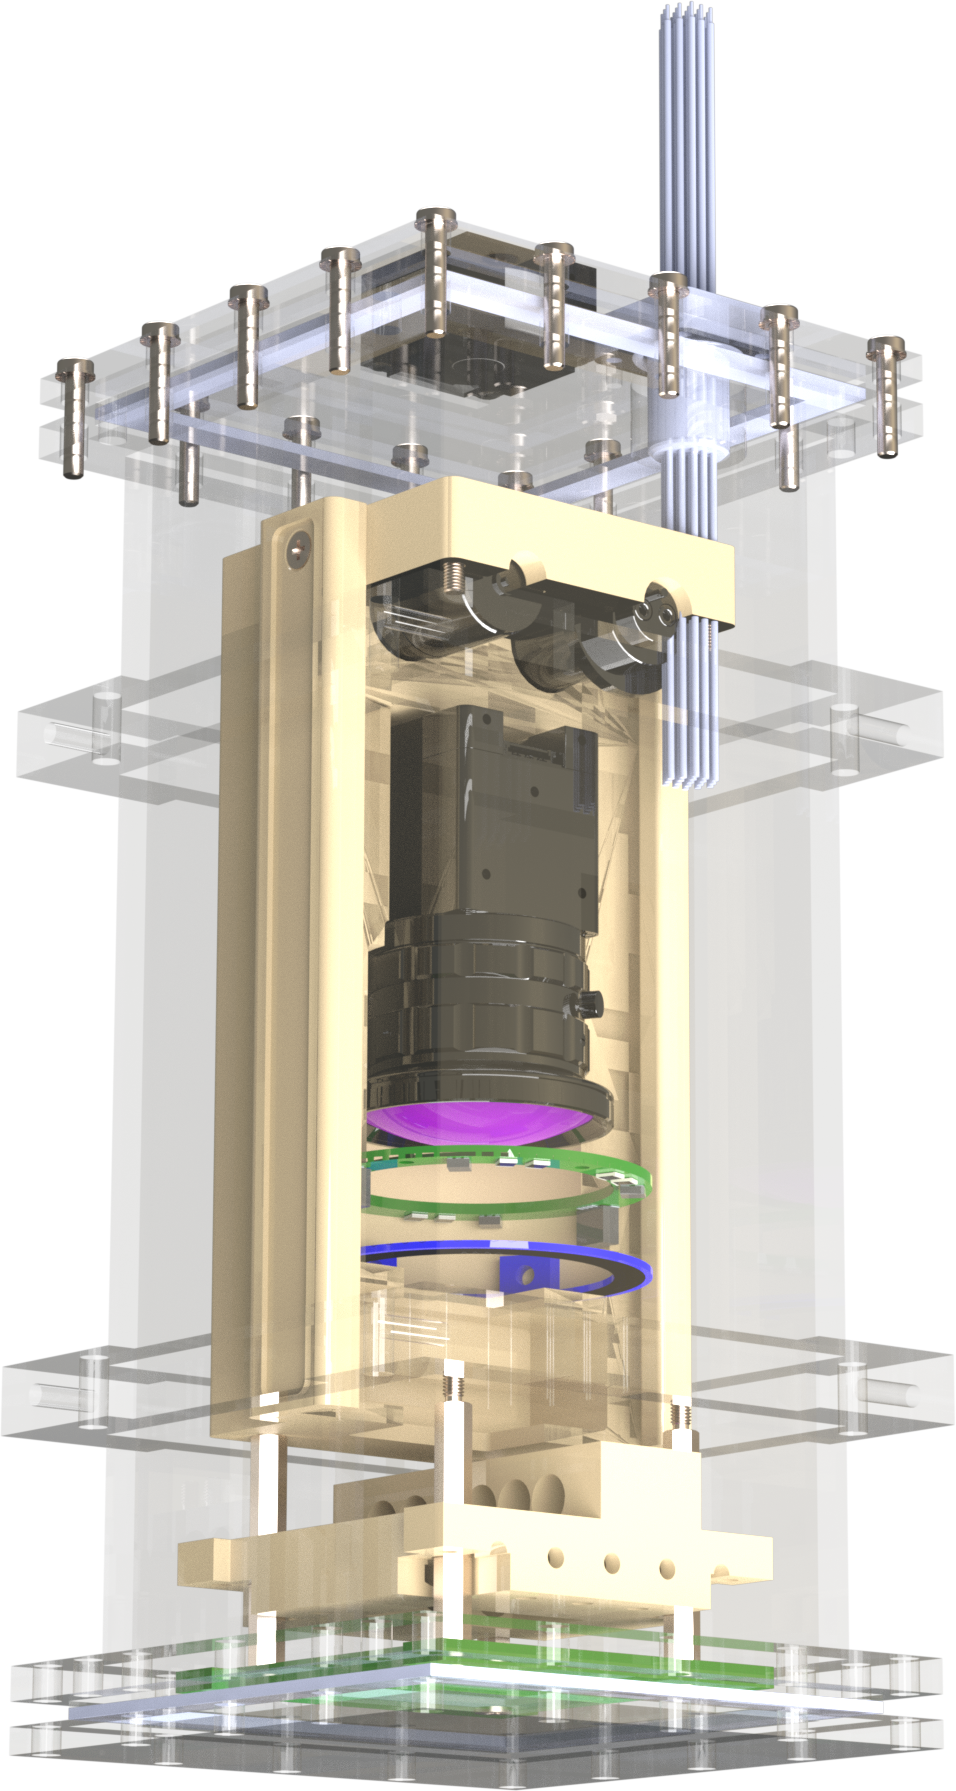
\includegraphics[width=.9\textwidth]{Glass_Payload}
	\caption{Διαφανής προβολή του δοχείου πειράματος και του εσωτερικού του}
	\label{fig:container}
\end{marginfigure}

Το πείραμα επιβάλλει κάποιους περιορισμούς στο σχεδιασμό του \ac{FDIR}:
\begin{enumerate}
	\item \textbf{Διακοπή} \g{ενός από τα τρία 72ωρα υποπειράματα κατά τη διάρκεια της εκτέλεσης μπορεί να σημαίνει πλήρη απώλεια του υποπειράματος. Ο αντίκτυπος ενός τέτοιου γεγονότος εξαρτάται από τη διάρκεια και τη χρονική στιγμή της εμφάνισής του. Σε κάθε περίπτωση, επαρκής παρατηρησιμότητα θα επιτρέψει στο επίγειο πείραμα να μιμηθεί όσο το δυνατόν περισσότερο τις συνθήκες εντός τροχιάς.}
	\item \textbf{Το πάγωμα} των υγρών στο εσωτερικό του τσιπ και των σωλήνων μπορεί να οδηγήσει σε μόνιμη βλάβη της διάταξης. Ως εκ τούτου, μπορεί να απαιτηθεί η ενεργή θέρμανση ακόμη και κατά τη διάρκεια της ασφαλούς λειτουργίας, μετά την εκτέλεση του πρώτου υπο-πειράματος και την εισροή υγρού στο σύστημα. Αυτά τα χαρακτηριστικά επιβάλλουν περαιτέρω περιορισμούς στην ελάχιστη διαθεσιμότητα του συστήματος, ανάλογα με τις περιβαλλοντικές συνθήκες.
\end{enumerate}

\begin{figure*}
	\centering
	\caption[Το τσιπ μικρορευστομηχανικής και ο διαχωρισμός του σε 3 επιμέρους υποπειράματα και 1 γραμμή δοκιμής]{Το τσιπ μικρορευστομηχανικής και ο διαχωρισμός του σε 3 επιμέρους υποπειράματα και 1 γραμμή δοκιμής. Οι είσοδοι των υγρών φαίνονται στην αριστερή πλευρά του τσιπ, ενώ οι έξοδοι στα δεξιά. \emph{Πράσινο:} στρώμα ροής. \emph{Μπλε:} στρώμα ελέγχου.}
	\label{fig:chip}
	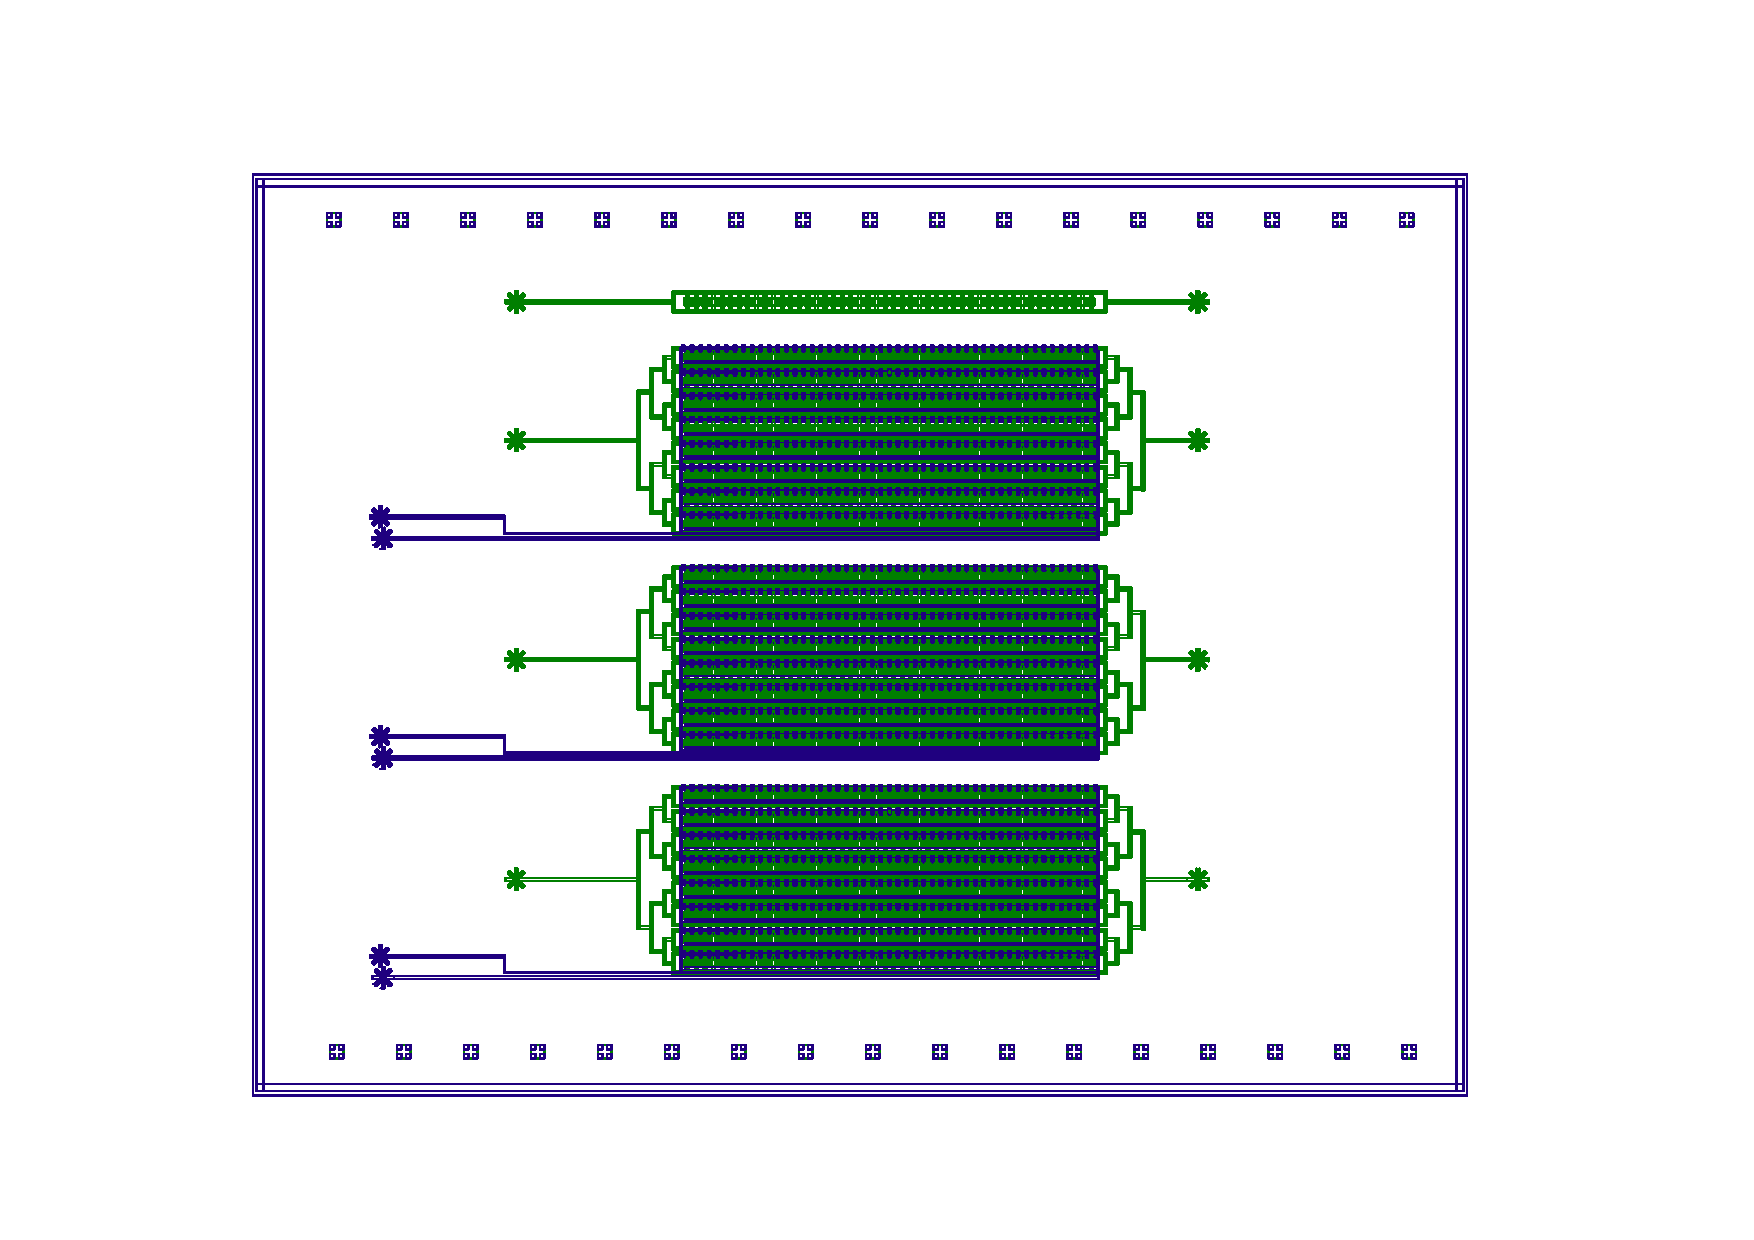
\includegraphics{final_chip.pdf}
	\begin{tikzpicture}[overlay]
	\draw[very thick,dashed,solarized-base01] (5,10.9) rectangle (-7,11.5) node[below right] {Δοκιμαστική};
	\draw[very thick,dashed,solarized-green] (5,7.85) rectangle (-7,10.8) node[below right] {Υποπείραμα $\alpha$};
	\draw[very thick,dashed,solarized-blue] (5,4.95) rectangle (-7,7.8) node[below right] {Υποπείραμα $\beta$};
	\draw[very thick,dashed,solarized-red] (5,2) rectangle (-7,4.9) node[below right] {Υποπείραμα $\gamma$};
	\end{tikzpicture}
\end{figure*}

\subsection{Thermal}


Η υποομάδα Thermal είναι υπεύθυνη για τη θερμική ανάλυση του δορυφόρου, όπου η εισερχόμενη ηλιακή ακτινοβολία συνδυάζεται με την απαγωγή θερμότητας των υποσυστημάτων, με σκοπό τον προσδιορισμό των χειρότερων θερμοκρασιών που αντιμετωπίζει ο δορυφόρος, σε θερμές και ψυχρές συνθήκες.

Τα αποτελέσματα της θερμικής ανάλυσης οδηγούν συνήθως στην εφαρμογή παθητικών ή ενεργητικών μεθόδων θερμικού ελέγχου. Ειδικότερα στο AcubeSAT, χρησιμοποιούνται 3 ηλεκτρονικά ελεγχόμενα θερμαντικά σώματα για τις μπαταρίες, το πειραματικό τσιπ και τις βαλβίδες.

\subsection{Trajectory}

Η υποομάδα Trajectory είναι υπεύθυνη για την ανάλυση της τροχιάς του διαστημικού σκάφους, την αποτίμηση των επιπτώσεων της ακτινοβολίας, τη συμμόρφωση του δορυφόρου με τους κανονισμούς για τα διαστημικά σκουπίδια και την εκτίμηση της διάρκειας ζωής του σε τροχιά.

Οι απαιτήσεις του AcubeSAT δεν υπαγορεύουν τη χρήση προωθητήρων, πράγμα που σημαίνει ότι η τροχιά του δορυφόρου καθορίζεται αποκλειστικά από την εκτόξευση και δεν μπορεί να τροποποιηθεί κατά την πτήση. Καθώς πληροφορίες για την εκτόξευση είναι άγνωστες μέχρι κάποιο χρονικό διάστημα πριν από την παράδοση του δορυφόρου, εκτελείται ένα σύνολο αναλύσεων ευαισθησίας για τον προσδιορισμό των επιτρεπόμενων τροχιών. \autocite{MDO,retselis_acubesat_fmea_2020}
\begin{figure}
	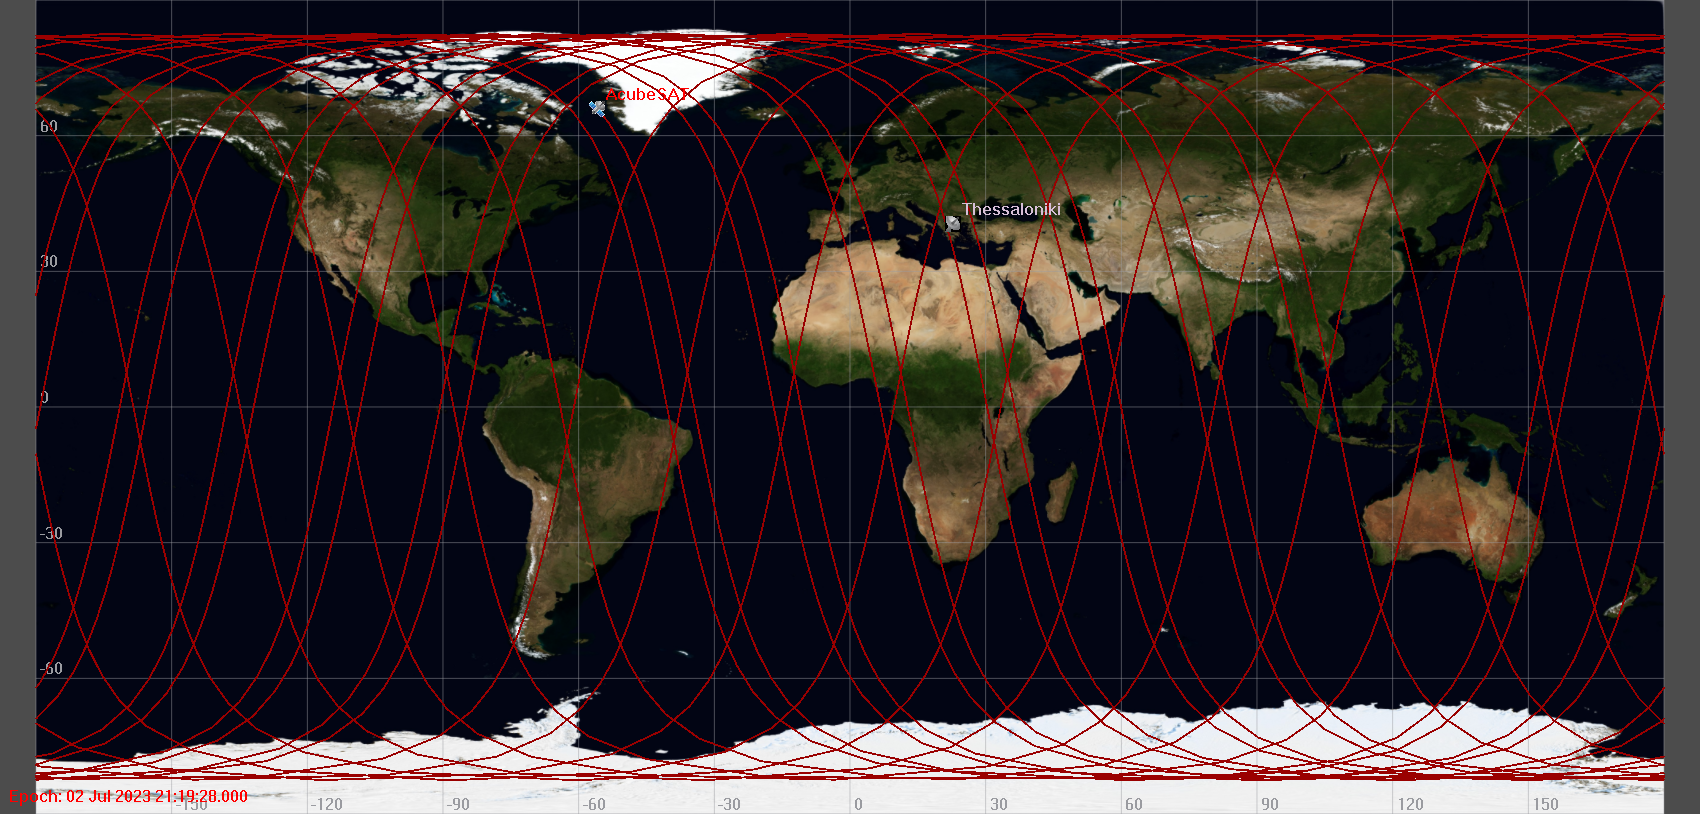
\includegraphics{GmatScreenShot_002}
	\caption[Επίγειο ίχνος μιας πιθανής τροχιάς του AcubeSAT]{Επίγειο ίχνος μιας πιθανής τροχιάς του AcubeSAT, σχεδιασμένο με χρήση του εργαλείου \acl{GMAT} της NASA}
	\label{fig:gmat}
\end{figure}

% Maybe add some info about the sensitivity results and LTAN value?
% No

\section{Χρησιμοποιούμενα εργαλεία}
\draft{Here we write a small paragraph about OCDT and other MBSE tools and utilities used by AcubeSAT or developed in-house...}

\chapter{Η φιλοσοφία \ac{FDIR} του SAVOIR}

\section{Το Πρότυπο Αξιοποίησης Πακέτων \acs{ECSS}}

\subsection{Οι Υπηρεσίες \acs{ECSS}}

\begin{figure}
	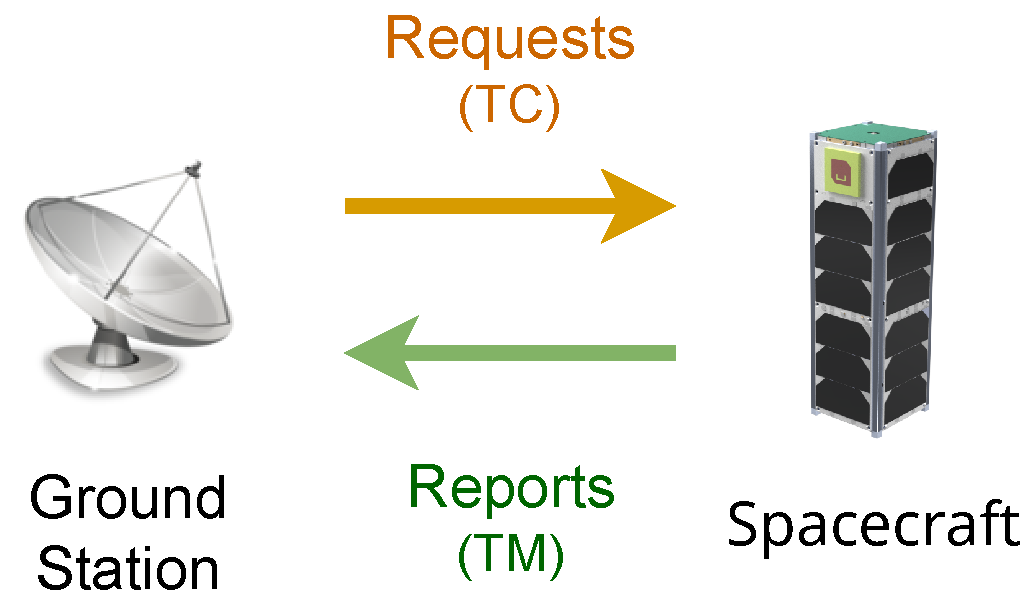
\includegraphics{ECSS-rq}
	\caption[][-1em]{The \ac{PUS} data transfer model}
	\label{fig:pusmodel}
\end{figure}

blablablab \autocite{ECSS-E-ST-70-41C,ECSS-E-70-41A,kaufeler_esa_standard_1994}

\begin{compactitem}
	\item \textbf{\texttt{ST[01]}: Request verification}
	
	Παρέχει αναφορές επιβεβαίωσης ή αποτυχίας για εκτελούμενες εντολές. Αυτή η υπηρεσία ουσιαστικά ενημερώνει τους χειριστές για την κατάσταση των \ac{TC} που αποστέλλονται στο διαστημικό σκάφος και αναφέρει τυχόν σφάλματα που συνέβησαν κατά την εκτέλεση.
	
	\item \textbf{\texttt{ST[02]}: Device access}
	
	Επιτρέπει την ενεργοποίηση, τον έλεγο και τη ρύθμιση των περιφερειακών συσκευών που δεν υποστηρίζουν το πρότυπο \ac{PUS}, αλλά βασίζονται σε απλούστερα πρωτόκολλα επικοινωνίας.
	
	\item \textbf{\texttt{ST[03]}: Housekeeping}
		
		Παράγει περιοδικές αναφορές που περιέχουν τιμές παραμέτρων. Η υπηρεσία αυτή ουσιαστικά συνθέτει τους περιοδικούς ραδιοφάρους (\textbf{\acs{RF} beacons}) του δορυφόρου, χωρίς προηγούμενο ερέθισμα.
		
		\item \textbf{\texttt{ST[04]}: Parameter statistics reporting}
		
		Επιτρέπει την αναφορά στατιστικών στοιχείων (ελάχιστο, μέγιστο, μέσος όρος, τυπική απόκλιση) για συγκεκριμένες παραμέτρους σε καθορισμένα χρονικά διαστήματα.
		
		\item \textbf{\texttt{ST[05]}: Event reporting}
		
		Δημιουργεί αναφορές όταν λαμβάνουν χώρα αξιοσημείωτα συμβάντα επί του σκάφους, όπως:
		\begin{compactitem}
			\item Αυτόνομες ενέργειες
			\item Ανιχνευμένες βλάβες ή ανωμαλίες
			\item Προκαθορισμένα βήματα μιας διαδικασίας
		\end{compactitem}
		
		\item \textbf{\texttt{ST[06]}: Memory management}
		
		Επιτρέπει την απευθείας ανάγνωση και εγγραφή σε μονάδες μνήμης. Αυτό μπορεί να είναι χρήσιμο για σκοπούς αποσφαλμάτωσης, ανάκτησης δεδομένων της αποστολής, ή φόρτωσης εντελώς νέου λογισμικού. Η υπηρεσία παρέχει επίσης τη δυνατότητα κατεβάσματος και ανεβάσματος αρχείων σε ένα σύστημα αρχείων (filesystem).
		
		\item \textbf{\texttt{ST[07]}: Task management} \emph{(καταργημένο)}
		
		Επιτρέπει τη διακοπή, την αναστολή ή την επανάληψη εργασιών λογισμικού σε περίπτωση έκτακτης ανάγκης. Η υπηρεσία αυτή έχει αφαιρεθεί από το πρότυπο και παρατίθεται για ιστορικούς λόγους.
		
		\item \textbf{\texttt{ST[08]}: Function management}
		
		Παρέχει τη δυνατότητα εκτέλεσης προκαθορισμένων ενεργειών που μπορούν να λάβουν περαιτέρω παραμέτρους. Οι ενέργειες αυτές μπορεί να αντιστοιχούν σε πειραματικές διαδικασίες, γενικότερες λειτουργίες ή οτιδήποτε άλλο.
		
		\item \textbf{\texttt{ST[09]}: Time management}
		
		Επιτρέπει την περιοδική αναφορά της τιμής του ρολογιού του CubeSat, για σκοπούς παρατηρησιμότητας και συσχέτισης.
		
		\item \textbf{\texttt{ST[10]}: Time packet} \emph{(καταργημένο)}
		
		Χρησιμοποιήθηκε στο παρελθόν για την παροχή πληροφοριών ρολογιού. Η υπηρεσία αυτή έχει αφαιρεθεί από το πρότυπο και παρατίθεται για ιστορικούς λόγους.
		
		\item \textbf{\texttt{ST[11]}: Time-based scheduling}
		
		Επιτρέπει στους χειριστές να προγραμματίζουν (\textbf{"time-tag"}) τηλεεντολές για εκτέλεση σε μελλοντικές χρονικές στιγμές, αντί για αμέσως.
		
		\item \textbf{\texttt{ST[12]}: On-board monitoring}
		
		Αυτή η υπηρεσία επιτρέπει τον έλεγχο των τιμών των παραμέτρων για να διασφαλιστεί ότι παραμένουν εντός ρυθμιζόμενων ορίων. Κάθε φορά που τα όρια παραβιάζονται, δημιουργείται ένα συμβάν (\texttt{ST[05]}) για περαιτέρω επεξεργασία.
		
		\item \textbf{\texttt{ST[13]}: Large packet transfer}
		
		Παρέχει μια μέθοδο τμηματοποίησης (segmentation) μηνυμάτων, για συμβολοσειρές που είναι πολύ μεγάλες για να χωρέσουν στο μέγιστο επιτρεπόμενο μήκος για \ac{TC} ή \ac{TM}.
		
		\item \textbf{\texttt{ST[14]}: Real-time forwarding control}
		
		Αυτή η υπηρεσία είναι υπεύθυνη για τον έλεγχο της παραγόμενης τηλεμετρίας που εκπέμπεται άμεσα προς το Σταθμό Βάσης.
		
		\item \textbf{\texttt{ST[15]}: On-board storage and retrieval}
		
		Η υπηρεσία αυτή επιτρέπει την αποθήκευση των παραγόμενων αναφορών, καθώς και την ανάκτησή τους όταν ο δορυφόρος περνάει επάνω από το Σταθμό Βάσης.
		
		\item \textbf{\texttt{ST[16]}: On-board traffic management} \emph{(deprecated)}
		
		Επιτρέπει την παρακολούθηση της κατάστασης και του φόρτου ενός διαύλου δεδομένων. Η υπηρεσία αυτή έχει αφαιρεθεί από το πρότυπο και παρατίθεται για ιστορικούς λόγους.
		
		\item \textbf{\texttt{ST[17]}: Test}
		
		Η υπηρεσία αυτή παρέχει απλές εντολές για ελέγχους υγείας του δορυφόρου.
		
		\item \textbf{\texttt{ST[18]}: On-board operations procedure}
		
		Επιτρέπει τη φόρτωση, τον έλεγχο (εκκίνηση, αναστολή, συνέχιση, διακοπή) και τη ρύθμιση των "operations procedures", οι οποίες είναι ακολουθίες εντολών γραμμένες σε κάποια ερμηνευμένει γλώσσα προγραμματισμού.
		
		\item \textbf{\texttt{ST[19]}: Event-action}
		
		Παρέχει τη δυνατότητα αυτόνομης εκτέλεσης \acp{TC} όταν λαμβάνει χώρα ένα συμβάν \texttt{ST[05]}.
		
		\item \textbf{\texttt{ST[20]}: On-board parameter management}
		
		Παρέχει τη δυνατότητα ανάγνωσης και αλλαγής τιμών των παραμέτρων του δορυφόρου. Οι παράμετροι είναι μερικές από τις πιο σημαντικές οντότητες που ορίζονται στο \acs{PUS} και μπορούν να αντιπροσωπεύουν:
		\begin{itemize}
			\item Βασικές ρυθμίσεις του συστήματος ή άλλων στοιχείων
			\item Μετρήσεις αισθητήρων και άλλες τιμές τηλεμετρίας
			\item Αποτελέσματα και διαγνωστικά του \ac{FDIR}
		\end{itemize}
		
		\item \textbf{\texttt{ST[21]}: Request sequencing}
		
		Επιτρέπει στους χειριστές να φορτώνουν σειρές \acp{TC} για να εκτελεστούν με διαδοχική σειρά.
		
		\item \textbf{\texttt{ST[22]}: Position-based scheduling}
		
		Παρέχει τη δυνατότητα εκτέλεσης \acp{TC} όταν το σκάφος φτάσει σε ένα συγκεκριμένο σημείο της τροχιάς του.
		
		\item \textbf{\texttt{ST[23]}: File management}
		
		Επιτρέπει την εκτέλεση διαχειριστικών εντολών σε τυχόν συστήματα αρχείων στον δορυφόρο, όπως \emph{αντιγραφή}, \emph{μετακίνηση}, \emph{διαγραφή}, ή \emph{κλείδωμα}.
\end{compactitem}

\section{Το πρότυπο SAVOIR}

\begin{figure*}[h]
	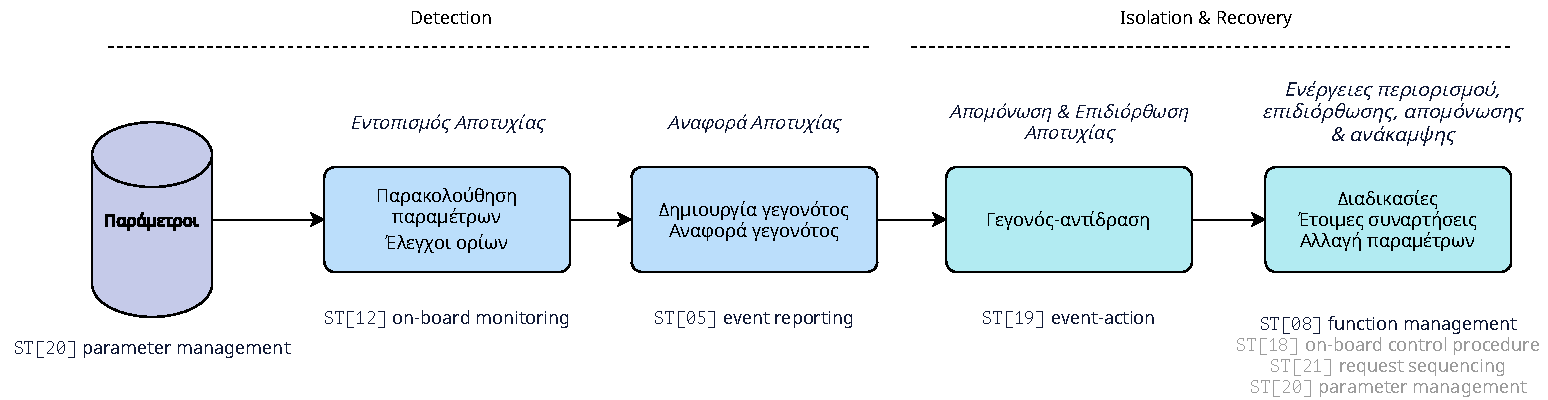
\includegraphics{../cdr/04 FMEA/media/FDIRpus}
	\caption{blablabla}
\end{figure*}

\chapter{\ac{FDIR} στο AcubeSAT}

\section{Βασικές αρχές του \ac{FDIR}}

\draft{\begin{itemize}
		\item The 7 AcubeSAT FDIR principles
		\item SAVOIR FDIR requirements and compliance
\end{itemize}}

\section{Μελέτη διαφορετικών αρχιτεκτονικών}

\begin{figure}
	\centering
	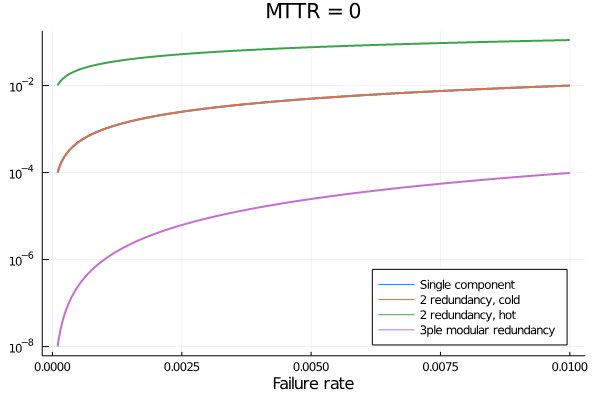
\includegraphics[width=.5\textwidth]{demoplot}
	\caption{\draft{Error rates}}
\end{figure}

\FloatBarrier
\section{Failure causes and recovery actions}

\subsection{Failure causes}

\subsection{Preventive actions}

\subsection{Corrective actions}

\section{\ac{FDIR} operating modes}
\label{sec:fdir_operating_modes}

\chapter{Practical demonstration of \ac{FDIR}}

As a proof of concept for AcubeSAT's \ac{FDIR} implementation, a practical setup to simulate the satellite's behaviour was prepared (\Cref{fig:block}). Key elements of the setup are:
\begin{compactitem}
	\item A Cortex-M7 \textbf{microcontroller}, used to simulate a \textbf{satellite subsystem}
	\item A number of redundant \textbf{sensors} used as the potential failure points
	\item The accompanying \textbf{software} that includes an implementation of the \ac{ECSS} services and the \ac{SAVOIR} \ac{FDIR} methodology
	\item A desktop computer, serving as the \textbf{ground station} to provide the necessary commanding and observing capabilities
\end{compactitem}

\begin{figure*}[h]
	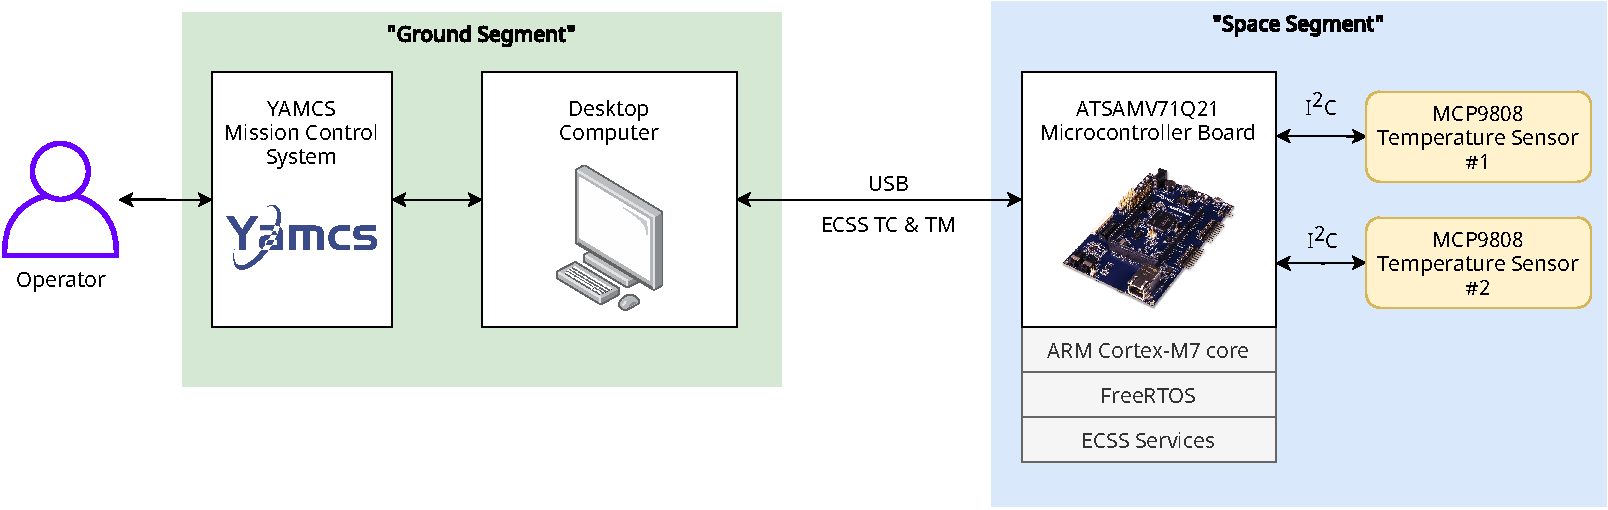
\includegraphics{SystemDescription}
	\caption{High-level block diagram of the demonstration system}
	\label{fig:block}
\end{figure*}

\section{System Description}

\subsection{Functionality}
\label{sec:tsvcd}

In order to emulate the most core functions of a spacecraft subsystem, we implemented a system with a single functional requirement:
\begin{quote}
	\texttt{RQ-010}: The system shall measure and report the ambient temperature.
\end{quote}

In order to justify implementing an \ac{FDIR} approach for this system, we will introduce a reliability requirement:
\begin{quote}
	\texttt{RQ-020}: No single failure on any measuring component shall lead to loss of system functionality
\end{quote}

The detailed design of this simple demonstration system is presented in the following sections, and was architected to match the functionality, interfaces, design and software of the AcubeSAT nanosatellite as much as possible.

\subsection{Hardware}

The centre of the demonstration system is the \ac{MCU} used to simulate the design and functionality of one of AcubeSAT's subsystems (\Cref{sec:obdh}). The selected \ac{MCU} is the Atmel \texttt{ATSAMV71Q21} hosted on the \foothref{https://www.microchip.com/Developmenttools/ProductDetails/ATSAMV71-XULT}{\texttt{ATSAMV71-XULT}} development board. This \ac{MCU} is functionally identical to the one that will be used in orbit, featuring a 32-bit ARM Cortex-M7 core with \SI{2}{\mebi\byte} of flash and \SI{384}{\kibi\byte} of \acs{SRAM} memory, and a maximum clock speed of \SI{300}{\mega\hertz}.

The \ac{MCU} is accompanied by two \textbf{temperature sensors} which are used to simulate subsystem components which are prone to failure. The selected sensor is the Microchip \foothref{https://www.microchip.com/wwwproducts/en/MCP9808}{\texttt{MCP9808}} which offers an accurate and frequent temperature readout over an \ac{I2C} bus. The maximum acquisition interval for the sensor is \SI{250}{\milli\second}.

\marginnote{%
\textbf{Cold redundancy:} Only one component is operating, while the other is not.

\textbf{Warm redundancy:} One component is operating fully, and the other is operating with reduced functionality.

\textbf{Hot redundancy:} Two or more simultaneously active parts operate in parallel. \parencite{SAVOIR-HB-003}
}

The two sensors are wired in a \textbf{hot-redundant} configuration, due to their extremely low operating power. The two sensors are connected to different \ac{I2C} buses, so that the failure of one bus will not affect the operation of the other sensor.

\paragraph{\acs{USB} interface} In order to receive \acl{TM} and transmit \acl{TC} to the demonstrative space segment, a \acs{USB} link with a desktop computer is integrated into the design. This link uses the \acs{UART} peripheral of the microcontroller, which solely transfers \acs{ECSS} messages between the microcontroller and the desktop. These messages include the typical \acs{TM} reports and \acs{TC} requests, but also log messages intended for diagnostic purposes.

As the \acs{UART} protocol does not offer packetisation facilities by default, \ac{COBS} encoding \autocite{cheshire_consistent_overhead_1997} is implemented for all transmitted messages.

\begin{figure*}[h]
	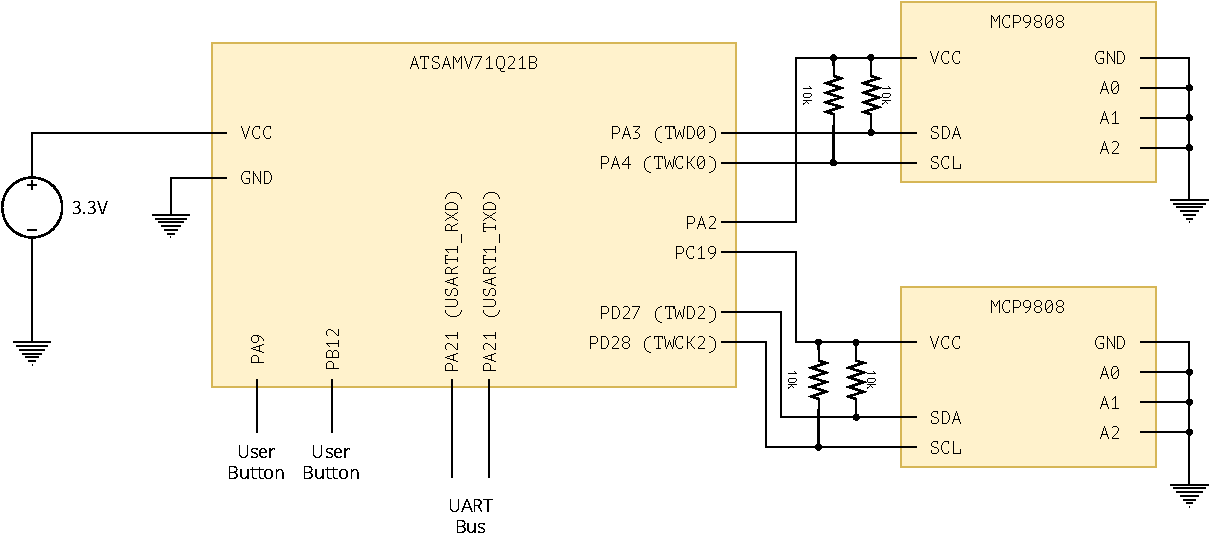
\includegraphics{ElectricalSchematic}
	\caption[Simplified electrical schematic of the implementation]{Simplified electrical schematic of the implementation. The two sensors are wired via \ac{I2C} with the necessary pull-up resistors. Their power is controlled directly by microcontroller outputs, allowing the user to completely cut the power of the sensors if needed. The \texttt{A} pins of the sensors are arbitrarily set to select the \ac{I2C} address of each device. The same address was used, as the two \ac{I2C} buses are separate. Decoupling capacitors, crystals and other boilerplate components are not shown, as they are already included in the \ac{MCU} development board.}
	\label{fig:schematic}
\end{figure*}

\paragraph{Connections}
The development board and sensors were laid out and connected directly. The sensor \acp{IC} were soldered on breakout \acp{PCB} which were manufactured based on Jaroslav Sýkora's design.\url{https://www.jsykora.info/2019/06/pcb-panel-\-of-smt-breakout-boards-soic-tssop-msop/}

\section{Software}

\subsection{Flight Segment}

All \ac{FDIR} operations and functionality are developed using the \textbf{C++} language\footnote{The \texttt{C++17} standard has been selected} on the \ac{MCU}. All developments rely on free and open source software which is freely available for download and modification. The \foothref{https://git-scm.com/}{Git} version control is used for all software projects.

The \ac{FDIR} functionality is structured around the \textbf{ECSS-E-ST-70-41C \ac{PUS} implementation created by the AcubeSAT team}\footnote{\url{https://gitlab.com/acubesat/obc/ecss-services}}, which offers a modular implementation of the standard utilising modern C++.

The \ac{MCU} software and business logic are built on \textbf{\foothref{https://www.freertos.org/}{Free\acs{RTOS}}}, a low-footprint real-time operating system targeted towards embedded devices. FreeRTOS provides the capability of safe concurrency, along with support for well-controlled tasks and a number of synchronisation primitives.

\begin{figure*}[h]
	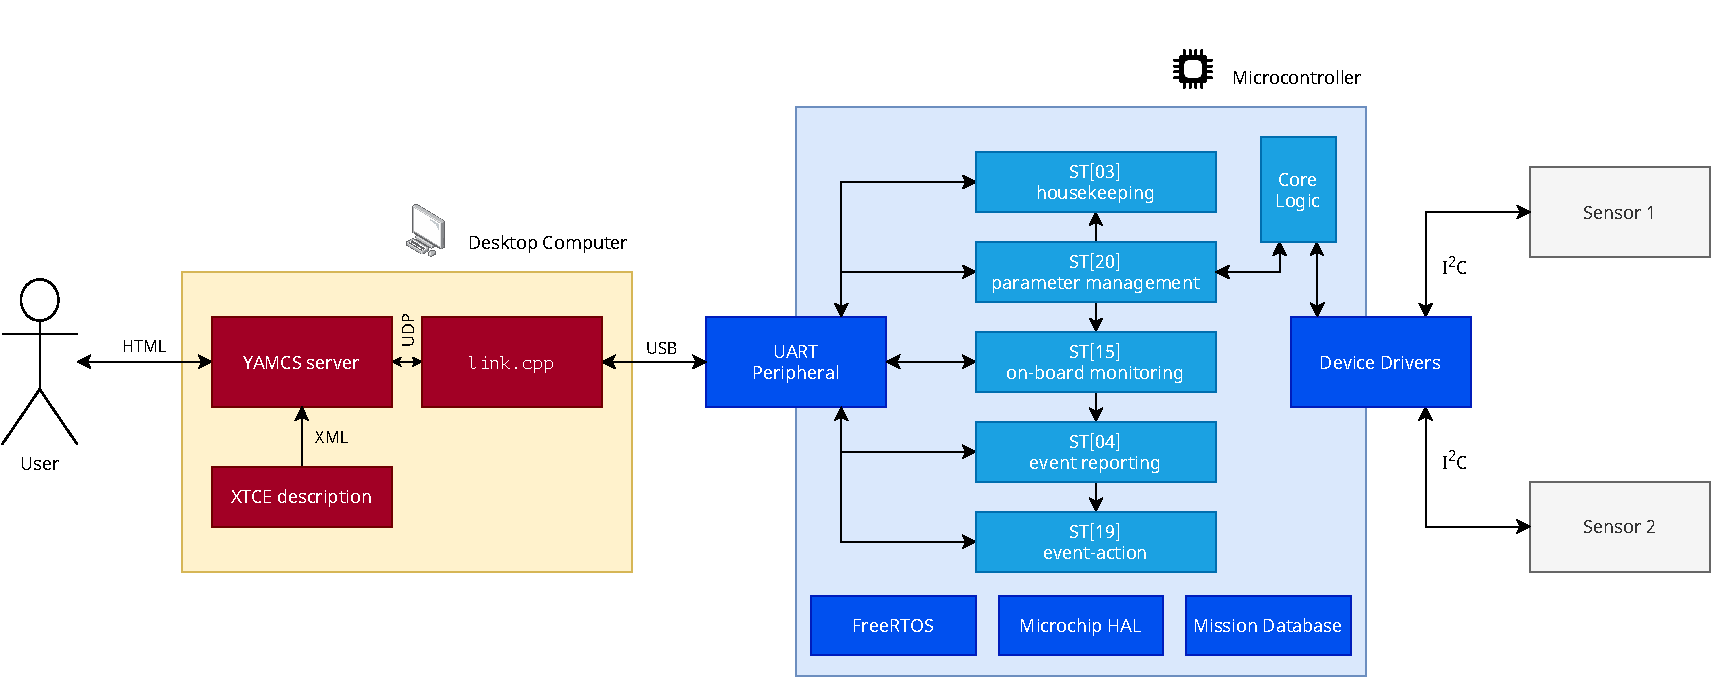
\includegraphics{SoftwareFlow}
	\caption{View of the software components and the data flow between them}
	\label{sec:softwareflow}
\end{figure*}

To ensure high reliability and a low resource footprint of the software, the following \textbf{constraints} are enacted in C++ development:
\begin{compactenum}
	\item Dynamic memory allocation\footnote{Use of \texttt{malloc}, \texttt{new} etc.} is banned completely from the code.
	\label{itm:malloc}
	\item \Cref{itm:malloc} means that standard C++ containers cannot be used. Instead, the \foothref{https://www.etlcpp.com/}{\acf{ETL}} is integrated in the software.
	\item "Expensive" features such as Run-Time Type Inference, Dynamic Casts or exceptions are also prohibited.
\end{compactenum}

The \foothref{https://www.microchip.com/en-us/development-tools-tools-and-software/embedded-software-center/mplab-harmony-v3}{MPLAB Harmony} \ac{HAL} and configurator are used to interface with all the \acs{MCU}'s peripherals. \foothref{https://www.jetbrains.com/clion/}{CLion} has been selected as the \acs{IDE}, along with the \foothref{https://cmake.org/}{CMake} build system.

All software developed in the scope of this thesis is available online, and listed in \Cref{tab:new_software}. The most critical parts of the developed software are expanded in \Cref{sec:source_code}. A summary of used libraries can also be found in \Cref{tab:old_software}.

\begin{table*}[h]
	\centering
	\caption[][5pt]{List of new software developed for this thesis}
	\label{tab:new_software}
	\begin{tabularx}{\textwidth}{@{}lXp{6cm}@{}}
		\toprule
		Library name & Description & URL \\ \midrule
		\textbf{\texttt{fdir-demo}} & Full microcontroller code for the demonstration & \small \url{https://github.com/kongr45gpen/fdir-demo} \\
		\textbf{\texttt{fdir-demo-yamcs}} & Ground segment software: files and source code for \acs{YAMCS} integration and \acs{MCU} communications & \small \url{https://github.com/kongr45gpen/fdir-demo-yamcs} \\
		\bottomrule
	\end{tabularx}
\end{table*}

\begin{table*}[h]
	\centering
	\vspace{2em}
	\caption[][5pt]{List of used "off-the-shelf" software libraries}
	\label{tab:old_software}
	\begin{tabularx}{\textwidth}{@{}lp{6cm}X@{}}
		\toprule
		Library name & Description & Modifications \\ \midrule
		\href{https://www.freertos.org/}{FreeRTOS} & Real-time operating system for embedded devices & \\
		\href{https://gitlab.com/acubesat/obc/ecss-services}{\texttt{ecss-services}} & C++ implementation of the ECSS-E-ST-70-41C \acl{PUS} %\autocite{ECSS-E-ST-70-41C} 
		& \small Missing services were implemented and some interface improvements were made to improve integration with the \acs{MCU}\newline\small\url{https://gitlab.com/kongr45gpen/ecss-services/-/tree/fdir}
		 \\
		 \href{https://www.etlcpp.com/}{\acs{ETL}}  & C++ library (including containers, algorithms and other utilities) for applications with embedded constraints &
		 \\
 		\href{https://github.com/yamcs/yamcs}{\acs{YAMCS}}  & Software framework for mission \& spacecraft control & %\autocite{cheshire_consistent_overhead_1997}
 		\\
		\href{https://github.com/cmcqueen/cobs-c}{\texttt{cobs-c}}  & Implementation of \ac{COBS} %\autocite{cheshire_consistent_overhead_1997}
		 & \\
		\bottomrule
	\end{tabularx}
\end{table*}

%\subsection{Space Segment}

%\subsection{Ground Segment}

\subsection{\ac{I2C} Failure Detection}

It is of interest to investigate how the hardware \ac{I2C} peripheral provided by the microcontroller can be used to monitor the symptoms of bus failure.

\begin{enumerate}
	\item \textbf{Microcontroller peripheral errors}
	
	\marginnote{To ensure detection of peripheral errors, it is important to make sure that the error status of the peripheral is not discarded after every operation. Interrupts and the \href{https://en.cppreference.com/w/cpp/language/attributes/nodiscard}{\mintinline{cpp}{[[nodiscard]]}} C++ feature are used to ensure that all errors are caught.}
	The microcontroller's \ac{I2C} peripheral is capable of generating an error whenever \emph{the communicating peripheral does not set the "acknowledge" bit}. Failure to set this bit might be a result of disconnection of the clock or data lines, failure of the bus, or non-operation of the peripheral itself.
	
	\item \textbf{Response timeout}
	
	For some adverse \ac{I2C} bus conditions, such as incorrectly chosen pull-up resistor values or large amounts of capacitive load, \ac{I2C} signal integrity may be lost (\Cref{subfig:i2c_clean}). This error is not detected by the microcontroller's peripheral directly, but can be diagnosed by adding a timeout to the sensor's data readouts.
	
	\item \textbf{Chip ID}
	
	\begin{margintable}
		\centering
		\caption{Read-only registers for the MCP9808}
		\label{tab:mcp9808readonly}
		\begin{tabularx}{\linewidth}{@{}lXl@{}}
			\toprule
			Address & Register Name & Value \\ \midrule
			\texttt{0x06} & Manufacturer ID & \texttt{0x0054} \\
			\texttt{0x07} & Device ID & \texttt{0x0400} \\ \bottomrule
		\end{tabularx}
	\end{margintable}
	
	It is possible that the sensor suffers a severe fault but is still able to respond to \ac{I2C} commands or set the \emph{acknowledge} bit. For this reason, a more rigid check of the sensor's status is performed before each temperature read: the \emph{permanently-set} registers of the peripheral contain values which, under nominal conditions, are hard-coded and will not change, barring hardware failure. If any value other than the expected one is return, the peripheral or the bus are assumed to have a fault.
\end{enumerate}

\begin{figure}[h]
	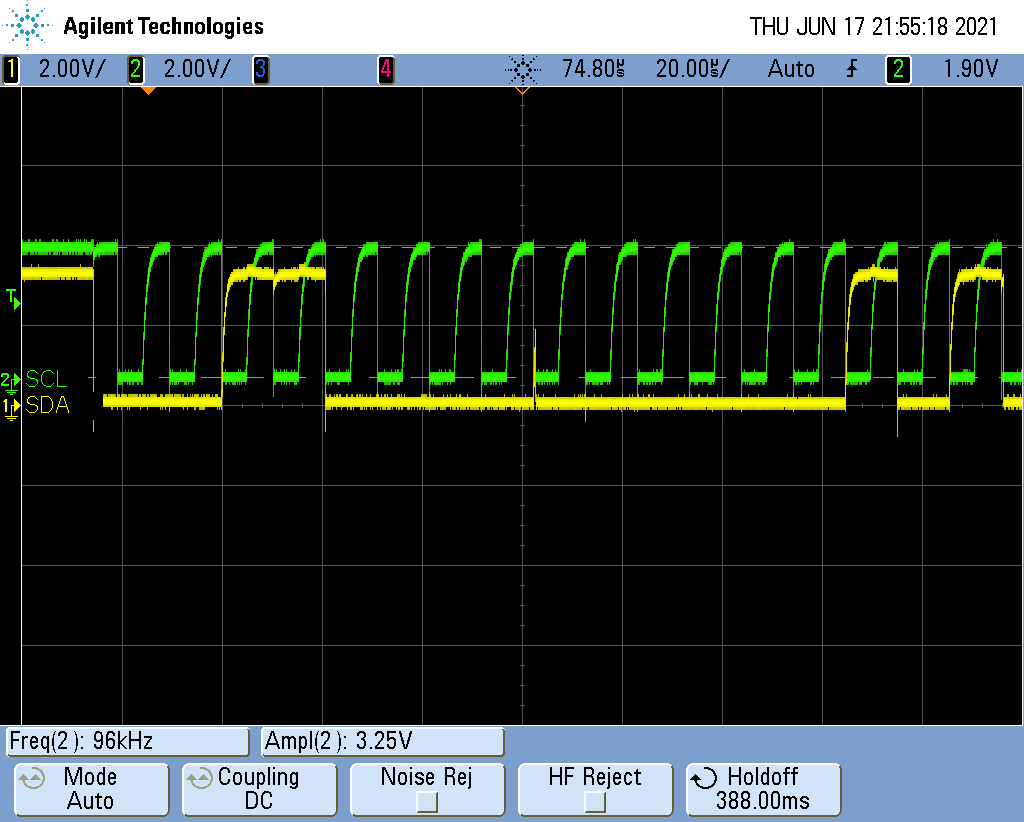
\includegraphics[trim={0 10cm 0 1.8cm},clip]{scope_1}
	\label{subfig:i2c_clean}
\end{figure}

\begin{figure}[h]
	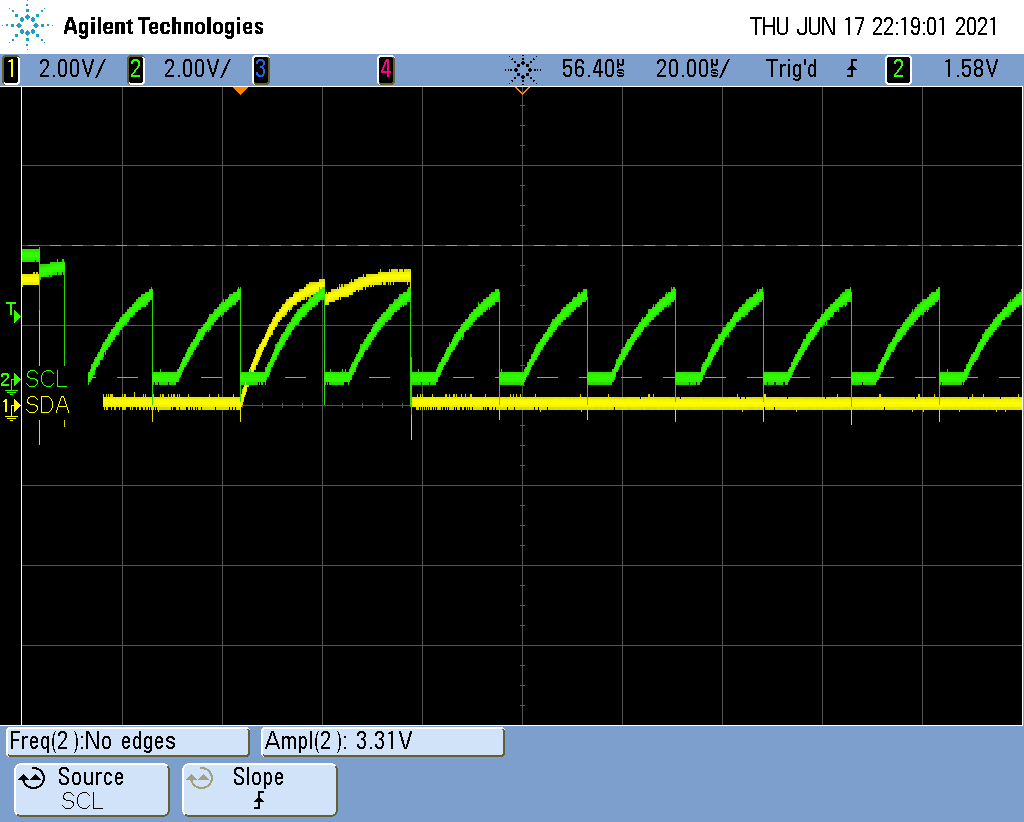
\includegraphics[trim={0 10cm 0 1.8cm},clip]{scope_5}
	\caption{blablabla}
	\label{subfig:i2c_dirty}
\end{figure}

\FloatBarrier

\subsection{Mission Control}

The ground segment desktop computer needs to parse received packets and send commands, as well as display information about the sensor measurements, \ac{FDIR} status and health of the connected flight system.

The \acs{YAMCS} \autocite{sela_yamcs_lightweight_2012} framework was selected to cover the aforementioned needs, and has been tailored to provide the capabilities needed for this demonstration.

The \ac{ECSS} protocol\autocite{ECSS-E-ST-70-41C} is not supported by \acs{YAMCS} by default. However, the necessary commands have been integrated into the system using the supported \ac{XTCE} specification.\autocite{simon_xtce_standard_2004} The source code of the integration can be found in \Cref{app:xtce}.

\begin{figure}[h]
	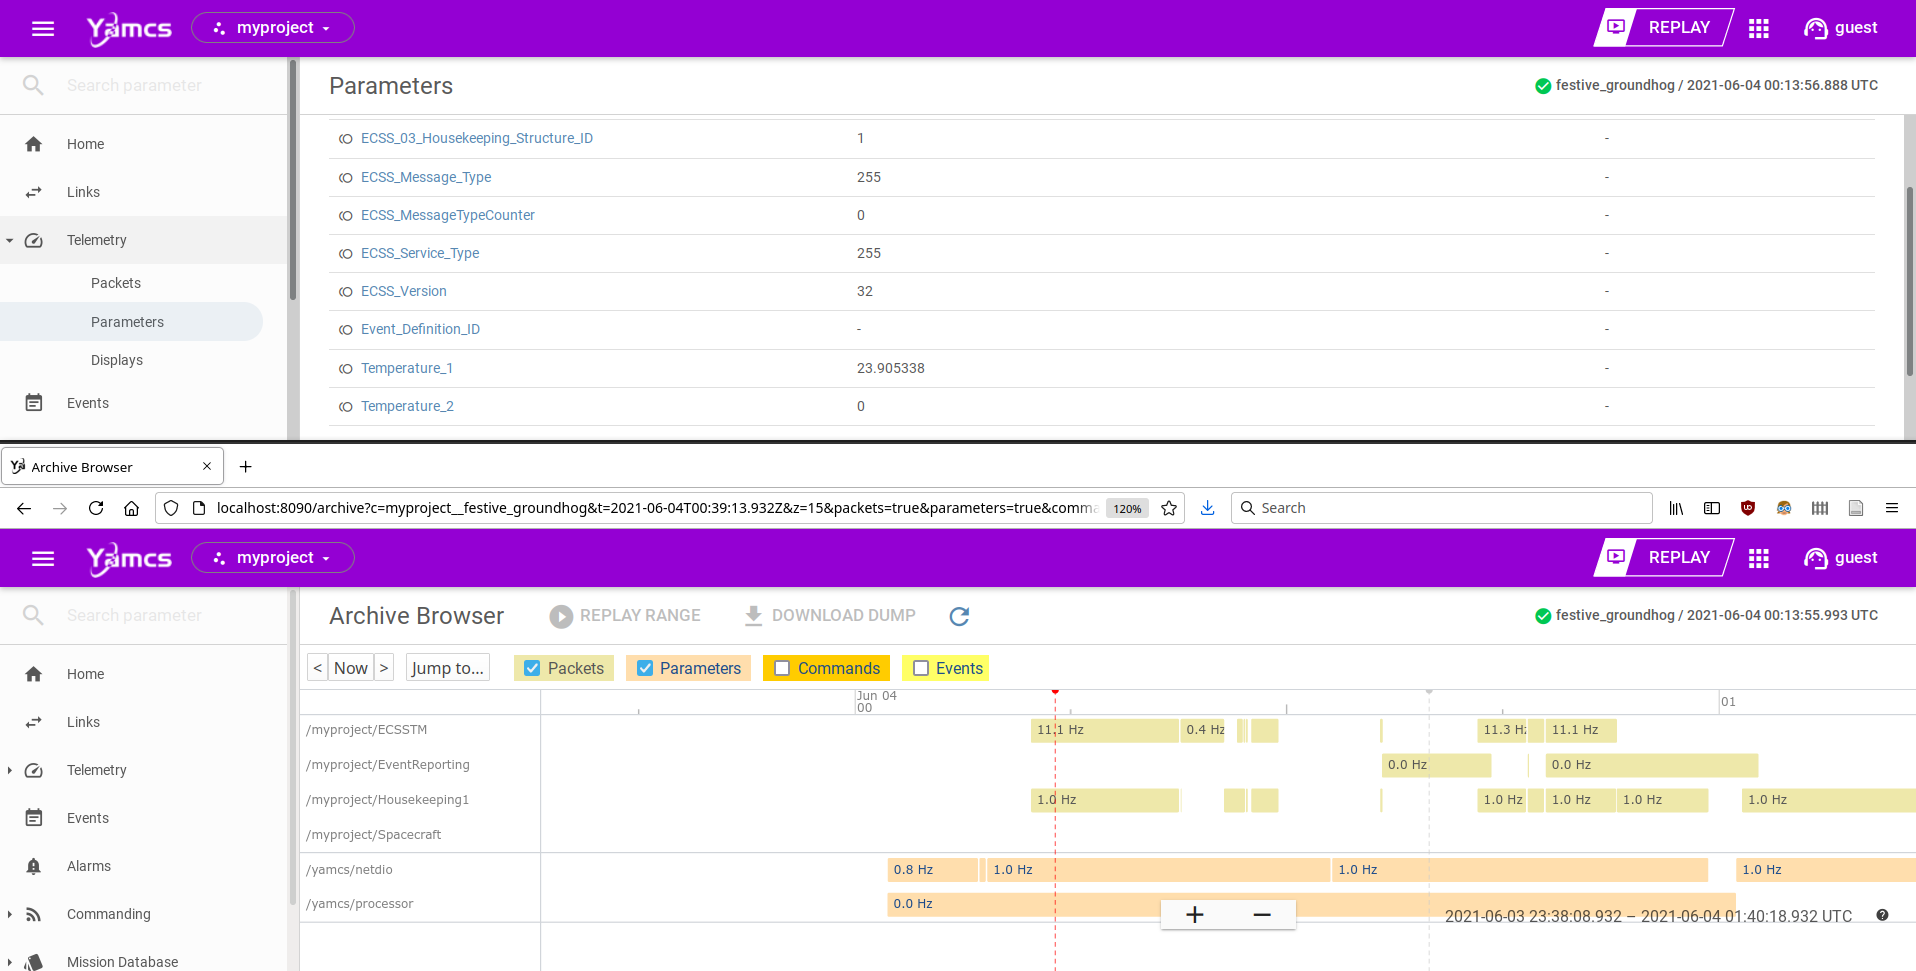
\includegraphics{screenshots/yamcs_replay}
	\caption{\acs{YAMCS} parameter and archive views}
\end{figure}

\subsection{\acs{PUS} database}

In 


\section{\ac{FDIR} setup}

The purpose of the test setup is to observe the response of the system to any failure of the two "vulnerable" temperature sensors. For this purpose, we will attempt to simulate every failure mode of each sensor, and design an \ac{FDIR} implementation that anticipates all those failures.

\marginnote{Double failures are not investigated in the scope of this document, as they are mostly considered only for launchers and manned missions \parencite{SAVOIR-HB-003}.}
As a required input for the \ac{FDIR} detailed design, a \ac{FMEA} analysis needs to be prepared for the system. All \ac{FMEA} performed follows the requirements of the ECSS-Q-ST-30-02C standard.\autocite{ECSS-Q-ST-30-02C} The analysis is based on the \ac{FMEA} performed for the AcubeSAT nanosatellite,\autocite{retselis_acubesat_fmea_2020} and can be seen in \Cref{tab:fmea} for the reduced system. All expected failure modes for the two sensors are investigated, as well as a failure mode for the entire system that can be detected by correctly-operating sensors. Each of those failure modes will be later verified by injecting software or hardware modifications.

\begin{table*}[h]
	\centering
	\caption[][10pt]{\acs{FMEA} on demonstration system}
	\label{tab:fmea}
	\begin{adjustbox}{width=1.05\textwidth,center}
	\begin{tabular}{@{}lL{4cm}L{2cm}L{1cm}L{4cm}L{2cm}L{4cm}L{1.5cm}L{3cm}@{}}
		\toprule
		\multicolumn{1}{l}{ID}                            & Failure Mode                     & Failure Cause(s)     & Mission Phase     & Failure effects: Local                                    & Failure effects: End effects & Failure Detection/Observable symptoms                                               & Severity level & Compensating provisions             \\ \midrule
		\multicolumn{9}{l}{Temperature sensor MCP9808 \#1}                                                                                                                                                                                                                                                                                                                                                               \\ \midrule
		\textbf{\texttt{F-010}}                                      & Temporary loss of function       & Intrinsic, Radiation & All & No temperature measurement from this sensor               & None                         & No communication via \acs{I2C}                                                            & 4              & Dual-redundant temperature sensor   \\
		\textbf{\texttt{F-020}}                                      & Permanent loss of function       & Intrinsic, Radiation & All & No temperature measurement from this sensor               & None                         & No communication via \acs{I2C}                                                            & 4              & Dual-redundant temperature sensor   \\
		\textbf{\texttt{F-030}}                                      & Short Circuit between power pins & Intrinsic, Radiation & All & No temperature measurement from this sensor               & None                         & No communication via \acs{I2C}                                                            & 4              & Current-limiting resistor           \\
		\textbf{\texttt{F-040}}                                      & Temporary Value Shift            & Intrinsic, Radiation & All & Incorrect temperature readings                            & None                         & Temperature difference between 2 redundant sensors bigger than a safety value  & 4              & Dual-redundant temperature sensor   \\
		\textbf{\texttt{F-050}}                                      & Permanent Value Shift            & Intrinsic, Radiation & All & Incorrect temperature readings                            & None                         & Temperature difference between 2 redundant sensors bigger than a safety value  & 4              & Dual-redundant temperature sensor   \\
		\textbf{\texttt{F-060}}                                      & \acs{I2C} bus pin output stuck         & Intrinsic, Radiation & All & Inability to communicate with both sensors & None                         & No communication via \acs{I2C} for all temperature sensors                                & 4              & Sensors wired on separate \acs{I2C} buses \\
		\midrule
		\multicolumn{9}{l}{Temperature sensor MCP9808 \#2}                        \\ \midrule
		\textbf{\texttt{F-070}}                                      & Temporary loss of function       & Intrinsic, Radiation & All & No temperature measurement from this sensor               & None                         & No communication via \acs{I2C}                                                            & 4              & Dual-redundant temperature sensor   \\
		\textbf{\texttt{F-080}}                                      & Permanent loss of function       & Intrinsic, Radiation & All & No temperature measurement from this sensor               & None                         & No communication via \acs{I2C}                                                            & 4              & Dual-redundant temperature sensor   \\
		\textbf{\texttt{F-090}}                                      & Short Circuit between power pins & Intrinsic, Radiation & All & No temperature measurement from this sensor               & None                         & No communication via \acs{I2C}                                                            & 4              & Current-limiting resistor           \\
		\textbf{\texttt{F-100}}                                      & Temporary Value Shift            & Intrinsic, Radiation & All & Incorrect temperature readings                            & None                         & Temperature difference between 2 redundant sensors bigger than a safety value & 4              & Dual-redundant temperature sensor   \\
		\textbf{\texttt{F-110}}                                      & Permanent Value Shift            & Intrinsic, Radiation & All & Incorrect temperature readings                            & None                         & Temperature difference between 2 redundant sensors bigger than a safety value  & 4              & Dual-redundant temperature sensor   \\
		\textbf{\texttt{F-120}}                                      & \acs{I2C} bus pin output stuck         & Intrinsic, Radiation & All & Inability to communicate with both sensors & None                         & No communication via \acs{I2C} for all temperature sensors                                & 4              & Sensors wired on separate \acs{I2C} buses \\ \midrule
		\multicolumn{9}{l}{Subsystem}                        \\ \midrule
		\textbf{\texttt{F-130}}                                      & Overheating       & Short circuit, Environmental & All & Vulnerable component failure             & Loss of subsystem functionality           & Measured temperature outside expected range  & 3              & Thermal analysis with uncertainty margins, overcurrent protection   \\
		\bottomrule
	\end{tabular}
	\end{adjustbox}
\end{table*}

\subsection{\ac{FDIR} detailed design}

\begin{figure*}[ht]
	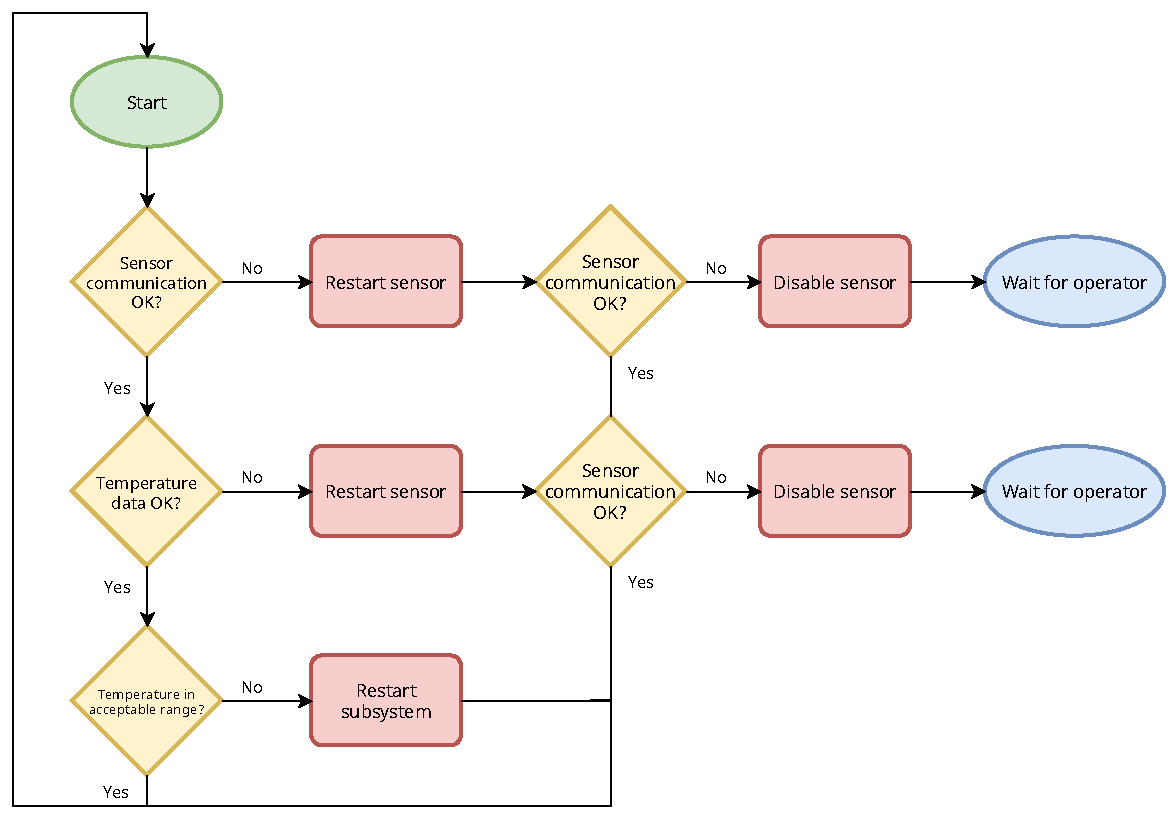
\includegraphics{TempSensorFDIR}
	\caption[Overview of the temperature sensor FDIR process]{Overview of the temperature sensor \ac{FDIR} process. For every process executed and failure detected, corresponding telemetry is generated as well.}
	\label{fig:fdirtemp}
\end{figure*}

The \ac{FDIR} of the sensors follows the hierarchical process described in \Cref{sec:fdir_operating_modes}, which is shown in \Cref{fig:fdirtemp} as tailored for the sensors.

The approach acts using the following steps, which are constantly being executed in the background:
\marginnote{For this demonstration, we will not investigate failures of the microcontroller itself and its internals. Refer to \parencite{retselis_acubesat_fmea_2020} for AcubeSAT's \acs{FMEA} and \acs{HSIA} on the microcontrollers.}
\begin{compactenum}
	\item The \ac{I2C} bus health status is monitored. Any failure or lack of communication indicates a failure in the sensor's electronics.
	\item The temperature output of the sensors is monitored. Any values which are outside the bounds of the physically possible thermal conditions are considered to indicate sensor or communication failures. Any values outside the operational limits of the subsystem's electronics are considered to indicate overheating and lead to a subsystem restart.
	\item In order to recover from the failures, first a restart of the sensor is attempted. If the erroneous values still persist, then the sensor cannot recover from the failure, but is just isolated and disabled instead.
\end{compactenum}

\clearpage
\paragraph{\acl{HSIA}}

After defining the possible failure modes and logic of the system, we are ready to analyse each entry to provide the correct software inputs to implement the required \ac{FDIR}. More specifically, for each failure, the following must be defined: \autocite[84]{SAVOIR-HB-003}
\begin{compactitem}
	\item Parameters to be monitored for detection
	\item Value ranges to be used to warn that a parameter is exceeding a specified range
	\item Isolation and reconfiguration actions to prevent failure propagation and, if possible, bring the system to a well operating state
\end{compactitem}

The above information is listed in the \acf{HSIA} table, which links each failure (identified in the \acl{FMEA}) to the corresponding low-level software parameters (\Cref{tab:hsia}).

For the purposes of this demonstration, we will consider that all \ac{FMEA} items can lead to \emph{feared events}, i.e. that \ac{FDIR} will anticipate all identified possible failures.

The \ac{HSIA} adds the following significant pieces of information to the \ac{FMEA}:\autocite{ECSS-Q-ST-30-02C}
\begin{itemize}
	\item The \textbf{monitored parameters} and the \textbf{conditions} that trigger the recovery action.
	
	These are listed here in terms of \ac{PUS} parameters which can be easily identified and compared by software. This list is then linked to the corresponding \emph{\texttt{ST[12]} on-board monitoring} service definitions, listed in \Cref{tab:demo_monitoring}.
	
	It is important to note that no single out-of-bounds value can trigger a recovery action. This is recommended in order to prevent transient errors or temporary communication protocol issues from triggering an unnecessary response which might disable a well-functioning component.
	
	\marginnote{\textbf{Temporary failure}: Caused by events such as bit flips, noise or transients, and can be corrected without intervention, or with a simple restart/power-cycle.\par\textbf{Permament failure}: A failure (typically in hardware, e.g. due to latchups or short-circuits) that cannot be corrected autonomously.}
	The distinction between \emph{temporary} and \emph{permanent} failures is made by \textbf{counting the number of consecutive failures}. Before a permanent action to disable a sensor is enacted, at least 5 attempts to communicate must have failed.
	
	The use of 2 hot-redundant sensor also allows us to investigate the difference between the two temperatures to deduce the health of the produced data. If the absolute difference between the 2 values is too high, assuming the sensors are placed close enough together, an error condition is assumed. However, as triple modular redundancy was not implemented for this system, it is not possible to deduce which sensor has failed.
	
	\item The \textbf{failure recovery and isolation actions}.
	
	These are listed in terms of \ac{PUS} events (\emph{\texttt{ST[05]} event reporting}) and event-actions (\emph{\texttt{ST[19]} eventaction}), which are linked to \Cref{tab:demo_eventaction}.
	
	The selected recovery actions match the approach shown in \Cref{fig:fdirtemp}. Additionally, when it is not known which sensor has failed, a fail-safe approach of restarting or disabling both sensors is used.
\end{itemize}

\begin{table*}
	\centering
	\caption{HSIA table}
	\label{tab:hsia}
	\begin{tabular}{@{}lL{4cm}L{4cm}L{1cm}L{1cm}L{3.5cm}@{}}
		\toprule
		ID & Failure Mode & Monitored Parameters & Monitoring ID & Event ID & Failure Recovery Action \\ \midrule
		\multicolumn{6}{l}{Temperature sensor MCP9808 \#1} \\ \midrule
		
		
		
		\textbf{\texttt{F-010}} & Temporary loss of function & \(\texttt{T1\_Status} = \texttt{TIMEOUT}\) \newline for 2 times & 0 & 0 & Power-cycle sensor 1 \\
		\textbf{\texttt{F-020}} & Permanent loss of function & \(\texttt{T1\_Status} = \texttt{TIMEOUT}\) \newline for 5 times & 2 & 2 & Ignore sensor 1 values \\
		\textbf{\texttt{F-030}} & Short Circuit between power pins & \(\texttt{T1\_Status} = \texttt{TIMEOUT}\) \newline for 5 times & 2 & 2 & Ignore sensor 1 values \\[5ex]
		\textbf{\texttt{F-040}} & Temporary Value Shift & 
		\(
		\begin{cases}
			\left|\Delta T\right| & > \SI{20}{\celsius} \text{ or} \\
			T_1 &> \SI{100}{\celsius} \text{ or} \\
			T_1 &< \SI{-40}{\celsius}
		\end{cases}
		\) \newline for 2 times
		 & 4, 6 & 0, 4 & Power-cycle sensor 1 \\
		\textbf{\texttt{F-050}} & Permanent Value Shift & \(
		\begin{cases}
		\left|\Delta T\right| & > \SI{20}{\celsius} \text{ or} \\
		T_1 &> \SI{100}{\celsius} \text{ or} \\
		T_1 &< \SI{-40}{\celsius}
		\end{cases}
		\) \newline for 5 times & 7, 9 & 2, 5 & Ignore sensor 1 values \\[9ex]
		\textbf{\texttt{F-060}} & \acs{I2C} bus pin output stuck & \(\texttt{T1\_Status} = \texttt{TIMEOUT}\) \newline for 5 times & 2 & 2 & Ignore sensor 1 values \\ \midrule
		
		
		
		\multicolumn{6}{l}{Temperature sensor MCP9808 \#2} \\ \midrule
		
		
		
		\textbf{\texttt{F-070}} & Temporary loss of function & \(\texttt{T2\_Status} = \texttt{TIMEOUT}\) \newline for 2 times & 1 & 1 & Power-cycle sensor 2 \\
		\textbf{\texttt{F-080}} & Permanent loss of function & \(\texttt{T2\_Status} = \texttt{TIMEOUT}\) \newline for 5 times & 3 & 3 & Ignore sensor 2 values \\
		\textbf{\texttt{F-090}} & Short Circuit between power pins & \(\texttt{T2\_Status} = \texttt{TIMEOUT}\) \newline for 5 times & 3 & 3 & Ignore sensor 2 values \\[5ex]
		\textbf{\texttt{F-100}} & Temporary Value Shift & 
		\(
		\begin{cases}
		\left|\Delta T\right| & > \SI{20}{\celsius} \text{ or} \\
		T_2 &> \SI{100}{\celsius} \text{ or} \\
		T_2 &< \SI{-40}{\celsius}
		\end{cases}
		\) \newline for 2 times
		& 5, 6 & 1, 4 & Power-cycle sensor 2 \\
		\textbf{\texttt{F-110}} & Permanent Value Shift & \(
		\begin{cases}
		\left|\Delta T\right| & > \SI{20}{\celsius} \text{ or} \\
		T_2 &> \SI{100}{\celsius} \text{ or} \\
		T_2 &< \SI{-40}{\celsius}
		\end{cases}
		\) \newline for 5 times & 8, 9 & 3, 5 & Ignore sensor 2 values \\[9ex]
		\textbf{\texttt{F-120}} & \acs{I2C} bus pin output stuck & \(\texttt{T2\_Status} = \texttt{TIMEOUT}\) \newline for 5 times & 3 & 3 & Ignore sensor 2 values \\ \midrule
		
		
		
		\multicolumn{6}{l}{Subsystem} \\ \midrule
		
		
		
		\textbf{\texttt{F-130}} & Overheating & \(T_1 > \SI{40}{\celsius}\) or \(T_2 > \SI{40}{\celsius}\) & 10, 11 & 6 & Restart subsystem \\ \bottomrule
	\end{tabular}
	\vspace{2pt}
\end{table*}

\clearpage

\paragraph{Parameters}

After investigating the \acl{HSIA}, we can list the scalar parameters for the \emph{\texttt{ST[20]} parameter management} service\autocite{ECSS-E-ST-70-41C} (\Cref{tab:demo_params}).

Beyond the actual temperature values, we have included the \textbf{difference} (\(\Delta\)) between the two temperatures, since the \acs{PUS} standard does not provide ways to perform arithmetic calculations without hard-coded software. Additionally, the status of each sensor peripheral is included, which is an enumerated value.\footnote{One of \texttt{NOMINAL}, \texttt{TIMEOUT} or \texttt{DISABLED}} 

These parameters are telemetered to the ground segment and displayed to the user periodically, via the \emph{\texttt{ST[03]} housekeeping} \ac{PUS} service. However, during flight, the ground segment will not have constant access, since the satellite will not be visible from ground stations throughout its entire orbit.

\begin{table}[h]
	\centering
	\caption[List of \texttt{ST[20]} parameters]{List of \texttt{ST[20]} parameters\\R: Read-only\\RW: Read-write}
	\label{tab:demo_params}
	\begin{tabularx}{\textwidth}{@{}rlllX@{}}
		\toprule
		Param. ID & Parameter              & Units & Type & Type \\ \midrule
		0            & Temperature 1          & \si{\celsius}      & \texttt{float} & R     \\
		1            & Temperature 2          & \si{\celsius}      & \texttt{float} & R    \\
		2            & \(\Delta\) Temperature & \si{\celsius}      & \texttt{float} & R    \\
		3            & Temperature 1 Status         &       & Enumerated   & RW  \\
		4            & Temperature 2 Status         &       & Enumerated   & RW  \\
		5			 & Temperature 1+2 Status       &		& Enumerated   & R  \\ \bottomrule
	\end{tabularx}
\end{table}

\paragraph{On-board monitoring definitions}

After defining the parameters, the monitoring definitions that establish the acceptable and actionable ranges for each parameter should be outlined. These are then managed by the \emph{\texttt{ST[12]} on-board monitoring} \ac{PUS} service.

The \emph{check validity conditions} are important to mention in this case, as they use the three \emph{Status} parameters to prevent executing checks for disabled peripherals. As such, sensors that are not providing values due to hardware issues, \ac{FDIR} actions or operator intervention, will not be able to trigger \ac{FDIR} actions.

\begin{table*}[h]
	\centering
	\caption[List of \texttt{ST[12]} monitoring definitions][5pt]{List of \texttt{ST[12]} monitoring definitions. \(t\) and \(\Delta\) are used as placeholders for parameter values.}
	\label{tab:demo_monitoring}
	\begin{adjustbox}{width=\textwidth}
	\begin{tabular}{@{}L{1cm}L{2.5cm}L{2.8cm}L{2cm}L{2cm}L{2cm}ll@{}}
		\toprule
		&  & \multicolumn{2}{c}{Check validity condition} &  &  & \multicolumn{2}{c}{Check} \\ \cmidrule(lr){3-4} \cmidrule(l){7-8} 
		Definition ID & Monitored Parameter & Validity Parameter & Expected Value & Monitoring Interval & Repetition Number & Check Type & Criteria \\ \midrule
		0 & Temp. 1 Status &  &  & \SI{500}{\milli\second} & 2 & Expected Value & \(\neq\) \texttt{TIMEOUT} \\
		1 & Temp. 2 Status &  &  & \SI{500}{\milli\second} & 2 & Expected Value & \(\neq\) \texttt{TIMEOUT} \\
		2 & Temp. 1 Status &  &  & \SI{500}{\milli\second} & 5 & Expected Value & \(\neq\) \texttt{TIMEOUT} \\
		3 & Temp. 2 Status &  &  & \SI{500}{\milli\second} & 5 & Expected Value & \(\neq\) \texttt{TIMEOUT} \\
		\midrule
		4 & Temperature 1 & Temp. 1 Status & \texttt{NOMINAL} & \SI{500}{\milli\second} & 2 & Range & \( -\SI{40}{\celsius} < t < \SI{100}{\celsius} \) \\
		5 & Temperature 2 & Temp. 2 Status & \texttt{NOMINAL} & \SI{500}{\milli\second} & 2 & Range & \( -\SI{40}{\celsius} < t < \SI{100}{\celsius} \) \\
		6 & \(\Delta\) Temperature & Temp. 1+2 Status & \texttt{NOMINAL} & \SI{500}{\milli\second} & 2 & Range & \( -\SI{20}{\celsius} < \Delta < \SI{20}{\celsius} \) \\
		\midrule
		7 & Temperature 1 & Temp. 1 Status & \texttt{NOMINAL} & \SI{500}{\milli\second} & 5 & Range & \( -\SI{40}{\celsius} < t < \SI{100}{\celsius} \) \\
		8 & Temperature 2 & Temp. 2 Status & \texttt{NOMINAL} & \SI{500}{\milli\second} & 5 & Range & \( -\SI{40}{\celsius} < t < \SI{100}{\celsius} \) \\
		9 & \(\Delta\) Temperature & Temp. 1+2 Status & \texttt{NOMINAL} & \SI{500}{\milli\second} & 5 & Range & \( -\SI{20}{\celsius} < \Delta < \SI{20}{\celsius} \) \\
		\midrule
		10 & Temperature 1 & Temp. 1 Status & \texttt{NOMINAL} & \SI{500}{\milli\second} & 5 & Range & \( t < \SI{50}{\celsius} \) \\
		11 & Temperature 2 & Temp. 2 Status & \texttt{NOMINAL} & \SI{500}{\milli\second} & 5 & Range & \( t < \SI{50}{\celsius} \) \\ \bottomrule
	\end{tabular}
	\end{adjustbox}
\end{table*}

\paragraph{Event-action definitions}

The final part of the puzzle are the event-action definitions, which can be seen on \Cref{tab:demo_eventaction} and combine:
\begin{itemize}
	\item \ac{PUS} events (\texttt{ST[05]} service) which are automatically generated when an on-board monitoring definition goes out of limits
	\item \ac{PUS} event-action definitions (\texttt{ST[19]} service), which link every occurrence of an event to a stored \ac{TC} that is immediately executed.
	They define the \acs{FDIR} recovery actions.
\end{itemize}

All the aforementioned definitions can be easily modified by operators using single commands that affect the on-board stored \ac{PUS} database.

\begin{table}[h]
	\centering
	\caption{List of \texttt{ST[19]} event-action definitions}
	\label{tab:demo_eventaction}
	\begin{tabular}{@{}lL{2cm}L{7cm}@{}}
		\toprule
		Event ID & Monitoring Definitions & Action \\ \midrule
		0 & 0, 4 & Restart sensor 1 \\
		1 & 1, 5 & Restart sensor 2 \\
		2 & 2, 7 & Set sensor 1 status \( = \) \texttt{DISABLED} \\
		3 & 3, 8 & Set sensor 2 status \( = \) \texttt{DISABLED} \\
		4 & 6 & Restart all sensors \\
		5 & 9 & Set all sensors status \( = \) \texttt{DISABLED} \\
		6 & 10, 11 & Restart system \\ \bottomrule
	\end{tabular}
\end{table}

\clearpage
\section{\ac{FDIR} validation}

\subsection{Nominal operation}

During nominal operation, no failures are simulated. The system is connected to power and outputs \ac{ECSS} telemetry (\Cref{fig:yamcshousekeeping}), which includes parameter values parsed by (\Cref{fig:yamcsparameter}). Additionally, a log file is kept for diagnostic purposes (\Cref{fig:lognominal}). The system is compliant with its requirements (\Cref{sec:tsvcd}) and can transmit the temperature to the ground station as expected.

\begin{figure}
	\centering
	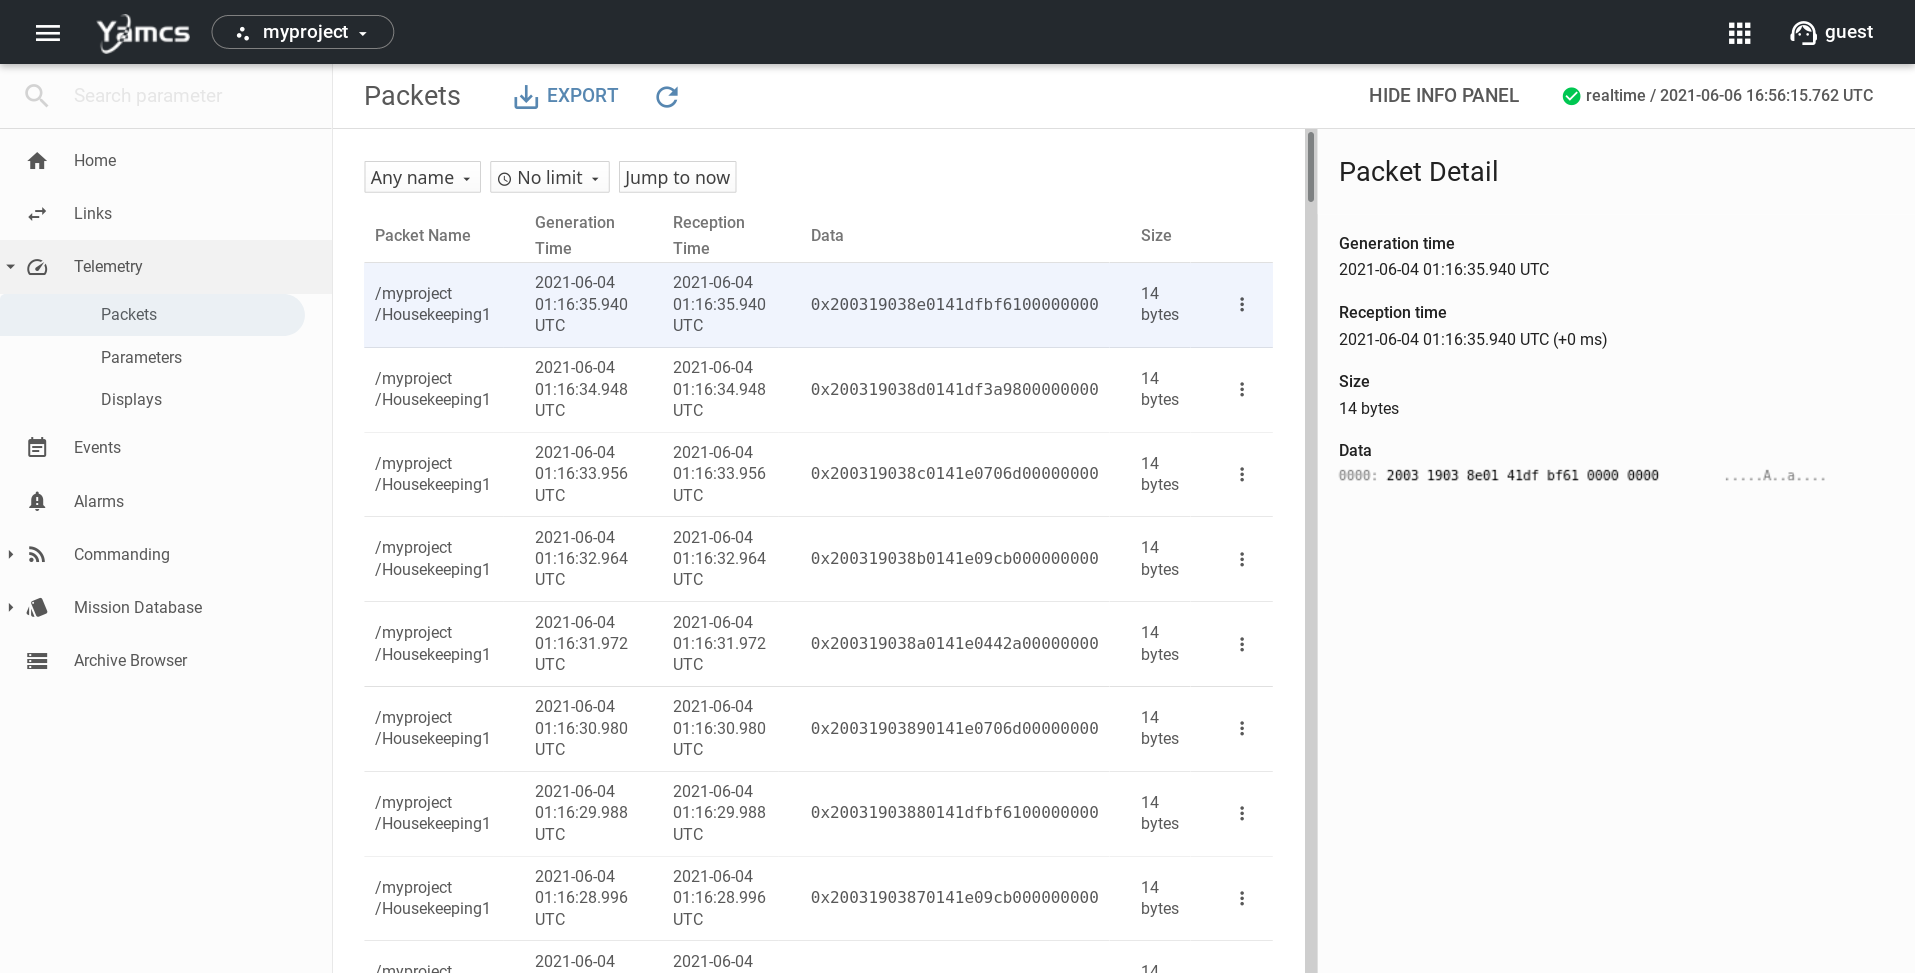
\includegraphics{media/screenshots/yamcs_housekeeping}
	\caption{View of housekeeping packets generated by the \acs{MCU} in \acs{YAMCS}}
	\label{fig:yamcshousekeeping}
\end{figure}

\begin{figure}[h]
	\centering
	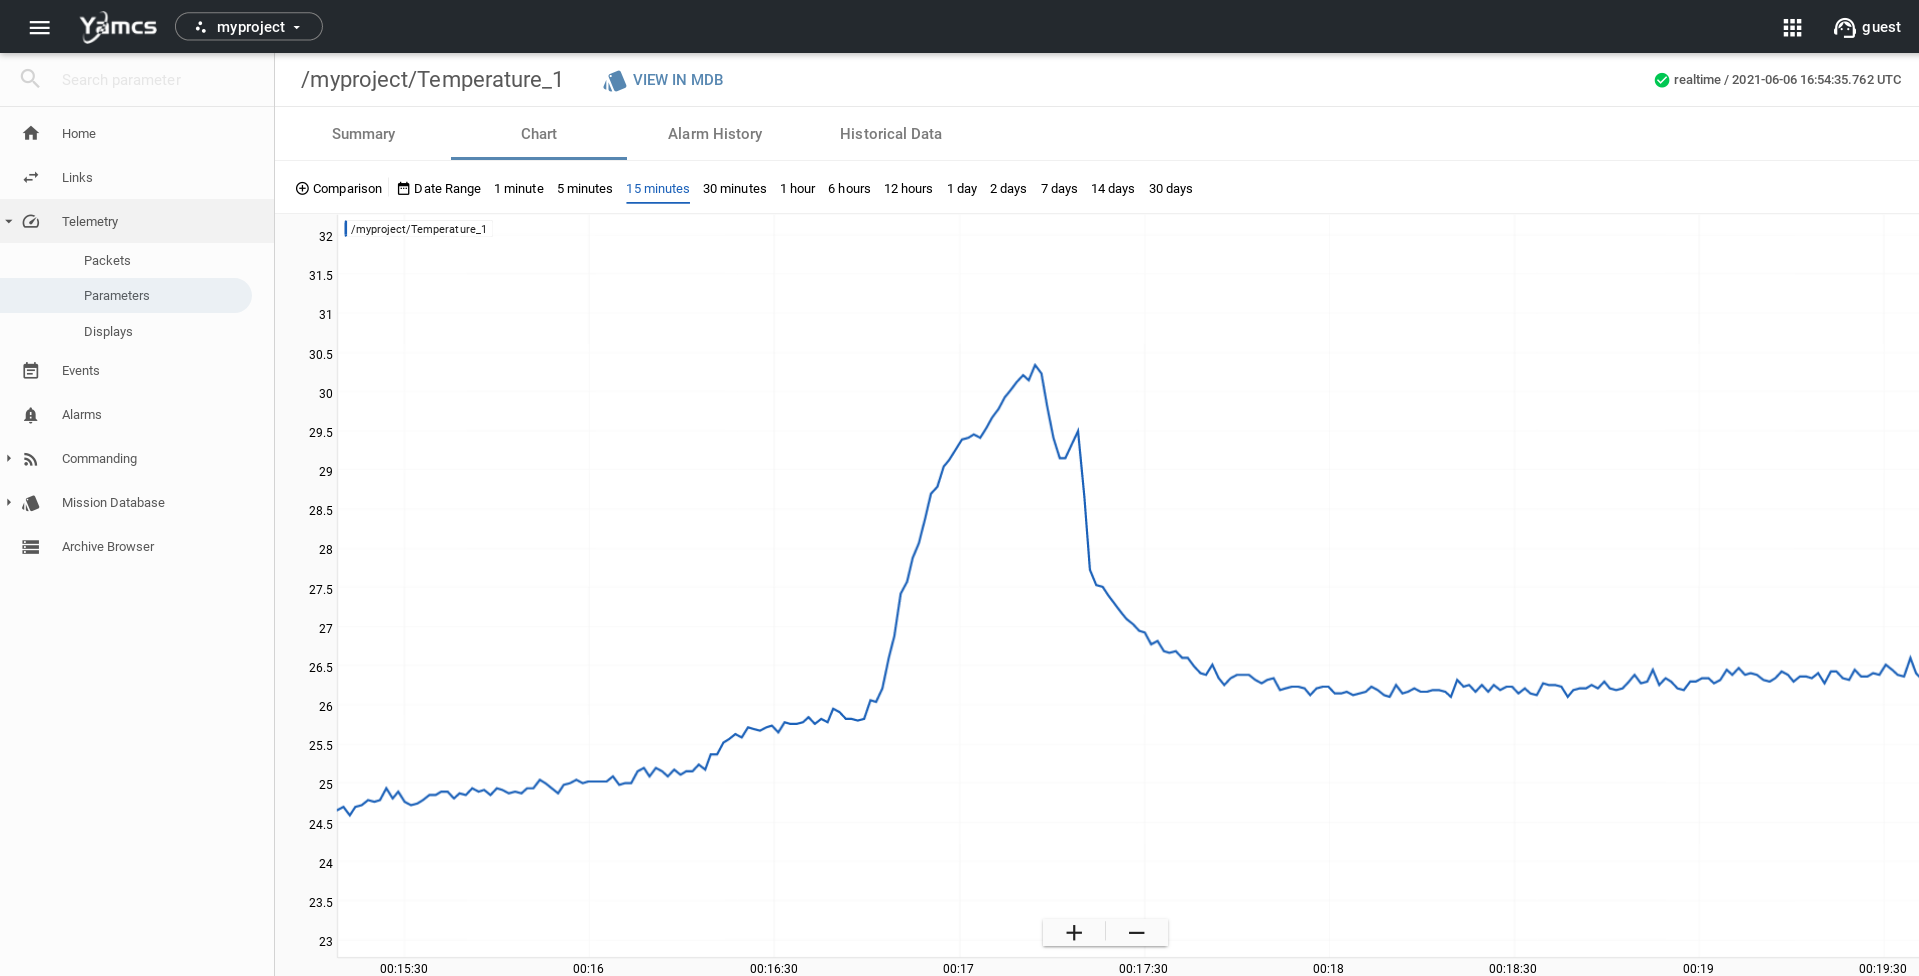
\includegraphics{media/screenshots/yamcs_parameter}
	\caption{View of one temperature parameter in \acs{YAMCS}}
	\label{fig:yamcsparameter}
\end{figure}

\begin{figure}
\begin{cminted}{text}
909601  [debug  ] T1 = 28.18
909701  [debug  ] T1 = 28.08
909801  [debug  ] T1 = 28.14
909901  [debug  ] T1 = 27.97
910000  [trace  ] New TM [3,25]
910001  [debug  ] T1 = 28.10
910101  [debug  ] T1 = 28.03
910201  [debug  ] T1 = 28.12
910301  [debug  ] T1 = 27.90
910401  [debug  ] T1 = 28.08
\end{cminted}
\caption[Log output during nominal operation]{Log output during nominal operation. The first number is the \ac{MCU} tick counter in milliseconds since boot.}
\label{fig:lognominal}
\end{figure}

\subsection{Simulation of failures}

The following methods were used to simulate each failure:
\begin{itemize}
	\item For component communication failures, each sensor was just physically disconnected from the system.
	\item For small changes in temperature, a hot air gun or other hot air source was pointed towards each sensor. Care was taken to not exceed the rated temperatures of the affected components.
	\item For changes in temperature which were impractical to simulate, the failure was injected in software, by manually modifying the variable.
	
	The two buttons present on the development board were used as a simple interface to "inject" extreme temperature values.
\end{itemize}

\subsection{Real-time modification of \ac{FDIR}}

The power of \acs{SAVOIR}'s \ac{FDIR} approach lies in the fact that the entire \ac{FDIR} concept can be safely modified via \ac{TC} without requiring any modifications or reuploads of the spacecraft's software. The application of the \acs{ECSS} services paradigm allows customising all on-board \ac{FDIR} functions and associated services using predefined \ac{TC} structures. In this section, \acs{ECSS} commands will be executed to demonstrate these capabilities and their control from the Ground Station.

The level of reconfigurability possible is defined by requirements listed in \parencite{ECSS-E-ST-70-11C,SAVOIR-HB-003}. The tailored version used for our experiments is listed in \Cref{tab:fdir-recon-rq}.

\begin{table*}[h]
	\centering
	\caption{\ac{FDIR} reconfigurability requirements}
	\label{tab:fdir-recon-rq}
	\begin{tabularx}{\textwidth}{@{}lXlL{4cm}@{}}
		\toprule
 		\# & Requirement & Service & Details \\ \midrule
		\texttt{RC-010} & The reporting of FDIR activities shall contain all information for failure analysis (e.g. time of occurrence, parameter out‐of‐limit, switching performed). & ST[12] on-board monitoring & Via periodic \emph{check transition reports} \\
		\texttt{RC-020} & The capability shall be provided to enable and to disable any on‐board FDIR function by telecommand. & ST[12] on-board monitoring & Via \emph{enable}/\emph{disable} \emph{parameter monitoring definitions} commands  \\
		\texttt{RC-030} & The capability shall be provided to add and delete parameters from the on‐board monitoring list. & ST[12] on-board monitoring & Via \emph{add}/\emph{delete} \emph{parameter monitoring definitions} commands  \\
		\texttt{RC-040} & The capability shall be provided to modify the failure recovery actions associated with each on-board monitoring definition. & ST[19] event-action & Via \emph{add}, \emph{delete}, \emph{enable} and \emph{disable} \emph{event-action definitions} commands \\ \bottomrule
	\end{tabularx}
\end{table*}

The \ac{YAMCS} platform was once again used to generate the wanted commands (\Cref{fig:yamcs_commands}).

\begin{figure}[h]
	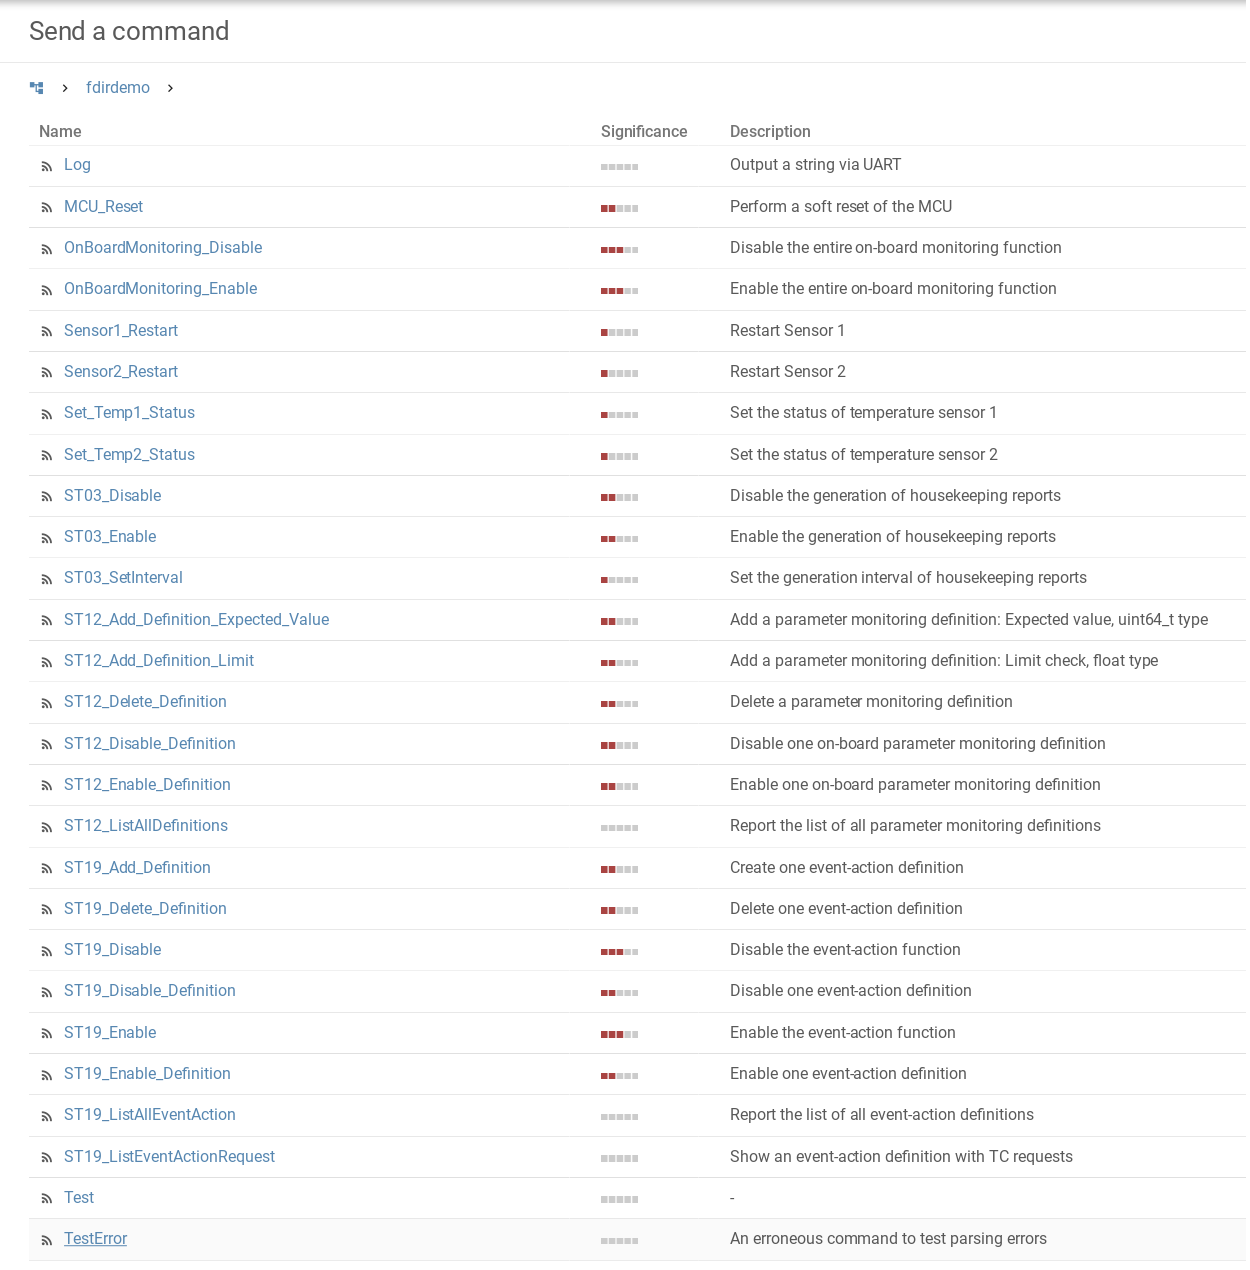
\includegraphics{screenshots/yamcs_commands.png}
	\caption{List of commands in the \acs{YAMCS} interface. These commands can initiate spacecraft actions, enable/disable sensors, or reconfigure the on-board \acs{ECSS} services databases. The list of commands is provided programmatically in \ac{XTCE} format (\Cref{app:xtce}).}
	\label{fig:yamcs_commands}
\end{figure}





\chapter{Conclusions and Future Work}

% Suggestions for standard:
% hard to play with parameters
% two validity conditions: safe mode etc. how to manage?
% derived parameters (e.g. Δ between sensors)
% event-action definition ID

\section{Future work}

%\backmatter
\appendix

\begin{fullwidth}
\printbibliography[heading=bibnumbered]
\end{fullwidth}


\printindex

\chapter{Source code}
\label{sec:source_code}

\setminted{
	bgcolor={},
	fontsize=\fontsize{9pt}{9pt}
}

%\begin{fullwidth}

\section*{\texttt{main.cpp}}

%\inputminted{cpp}{code/main.cpp}

\newpage
\section*{\texttt{xtce.xml}}
\label{app:xtce}

fixme

%\inputminted{xml}{code/xtce.xml}

%\end{fullwidth}

\end{document}

